%%%%%%%%%%%%%%%%%%%%%%%%%%%%%%%%%%%
%%%%%%%%% Modeling Chapter %%%%%%%%
%%%%%%%%%%%%%%%%%%%%%%%%%%%%%%%%%%%
\label{ch: modeling}

\par In order to understand, validate, and optimize the single cell impedance spectroscopy system, three models were implemented: an analytic impedance solution, finite element analysis simulations, and a circuit model. The analytic impedance solution was implemented to build a foundational understanding understanding of how basic IS systems behave, to optimize simple IS systems, and to validate FEA simulations. The finite element analysis expands upon the analytic solution to understand how the complex device geometry differentiates from the simple analytic impedance model geometry, and to inform optimized device designs. The circuit model was developed to validate the IS DAQ system, understand its shortcomings, and explore alternative measurement circuits.

%%%%%%%%%%%%%%%%%%%%%%%%%%%%%%%%%%%
%%%% Analytic Impedance Model %%%%%
%%%%%%%%%%%%%%%%%%%%%%%%%%%%%%%%%%%
\section{Analytic Single Cell Impedance Model}
\par For cell suspensions with low volume fractions, Maxwell's Mixture theory can model the electrical impedance of the system. The model is summarized in equations \ref{eqn: analyticImpedance} to \ref{eqn: cEpsParticle} below. 
\begin{equation}
    \Tilde{Z}_{mix} = \frac{1}{jw\Tilde{C}}
    \label{eqn: analyticImpedance}
\end{equation}
\begin{equation}
    \Tilde{C} = \Tilde{\epsilon}_{mix}G_f    
\end{equation}
\begin{equation}
    \Tilde{\epsilon}_{mix} = \Tilde{\epsilon}_m \frac{1 + 2\phi\Tilde{f}_{cm}}{1-\phi\Tilde{f}_{cm}}
\end{equation}
\begin{equation}
 \Tilde{f}_{cm} = \frac{\Tilde{\epsilon}_p - \Tilde{\epsilon}_{m}}{\Tilde{\epsilon}_p + 2\Tilde{\epsilon}_m}
\end{equation}
\begin{equation}
      \tilde{\epsilon}_p = \tilde{\epsilon}_{mem} 
      \frac{\gamma^3+2(\frac{\tilde{\epsilon}_i - \tilde{\epsilon}_{mem}}
      {\tilde{\epsilon}_i + 2\tilde{\epsilon}_{mem}})}{\gamma^3 - (\frac{\tilde{\epsilon}_i - \tilde{\epsilon}_{mem}}{\tilde{\epsilon}_i + 2\tilde{\epsilon}_{mem}})} \;\text{  with  } 
      \gamma = \frac{R + d}{R},
      \label{eqn: cEpsParticle}
\end{equation}

\par An explanation of these equations are given in section \ref{sec:maxwell_mixture_theory}. The values for $G_f$ (geometric constant) and $\phi$ (volume fraction) are dependent on the geometry of the system. In the following sections, solutions to both variables will be presented for the co-planar electrode configuration in figure \ref{fig:simplified_IS_models}.


 \begin{figure}[ht]
 \centering
 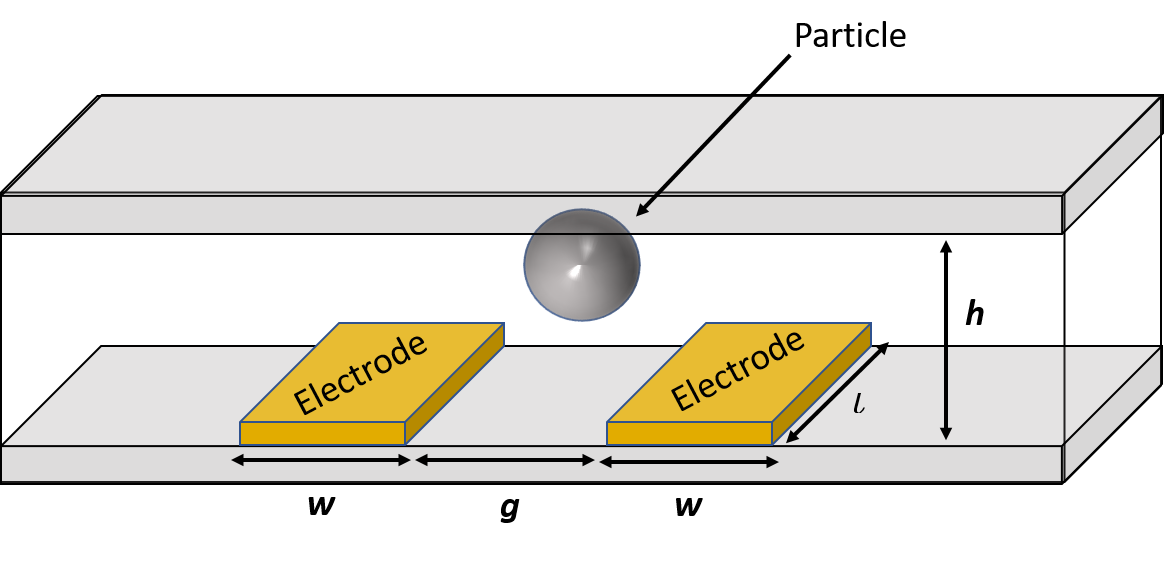
\includegraphics[width=0.7\textwidth]{images/cellAndElectrodes.png}
 \caption[Schematic diagram of simplified impedance sensor chamber.]{Schematic diagram of simplified impedance sensor chamber where w, $g$, and $l$ are the width, gap, and length of the electrodes respectively, and $h$ is the height of the chamber.}
 \label{fig:simplified_IS_models}
 \end{figure}


\subsection{Coplanar Electrode Cell Constant}
\label{sec: coplanarElectrodeCellConstant}
    \par The geometric constant is the inverse of the cell constant ($\kappa$). If the cell constant is thought of in terms of the resistive cell constant ($R=\kappa\rho$), then the geometric cell constant can be thought of as the capacitive cell constant ($C=G_f\epsilon$). If equations \ref{eqn: analyticImpedance} to \ref{eqn: cEpsParticle} were expressed in terms of complex conductivities rather than complex permittivities, the impedance of the mixture could be expressed as $\Tilde{Z}_{mix}=\frac{\kappa}{\Tilde{\sigma}}$. For the ideal parallel plate capacitor in figure \ref{fig:parallelCapacitorModel}, where the electric field is uniform, the geometric constant can be expressed as
    \begin{equation}
        (G_f)^{-1} = \kappa = \frac{d}{l\gamma},
        \label{eqn: cellConstants}
    \end{equation}
    \noindent where $d$ is the distance between the capacitors, $\gamma$ is the height of the capacitors, and $l$ is the length of the capacitors. This relation is discussed in further detail in section \ref{sec:electrode_cell_constant}. If the co-planar electrode geometry is mapped to the ideal parallel plate capacitor configuration, the ratio of $d$ and $\gamma$ can be derived. 

   \begin{figure}[ht]
        \centering
        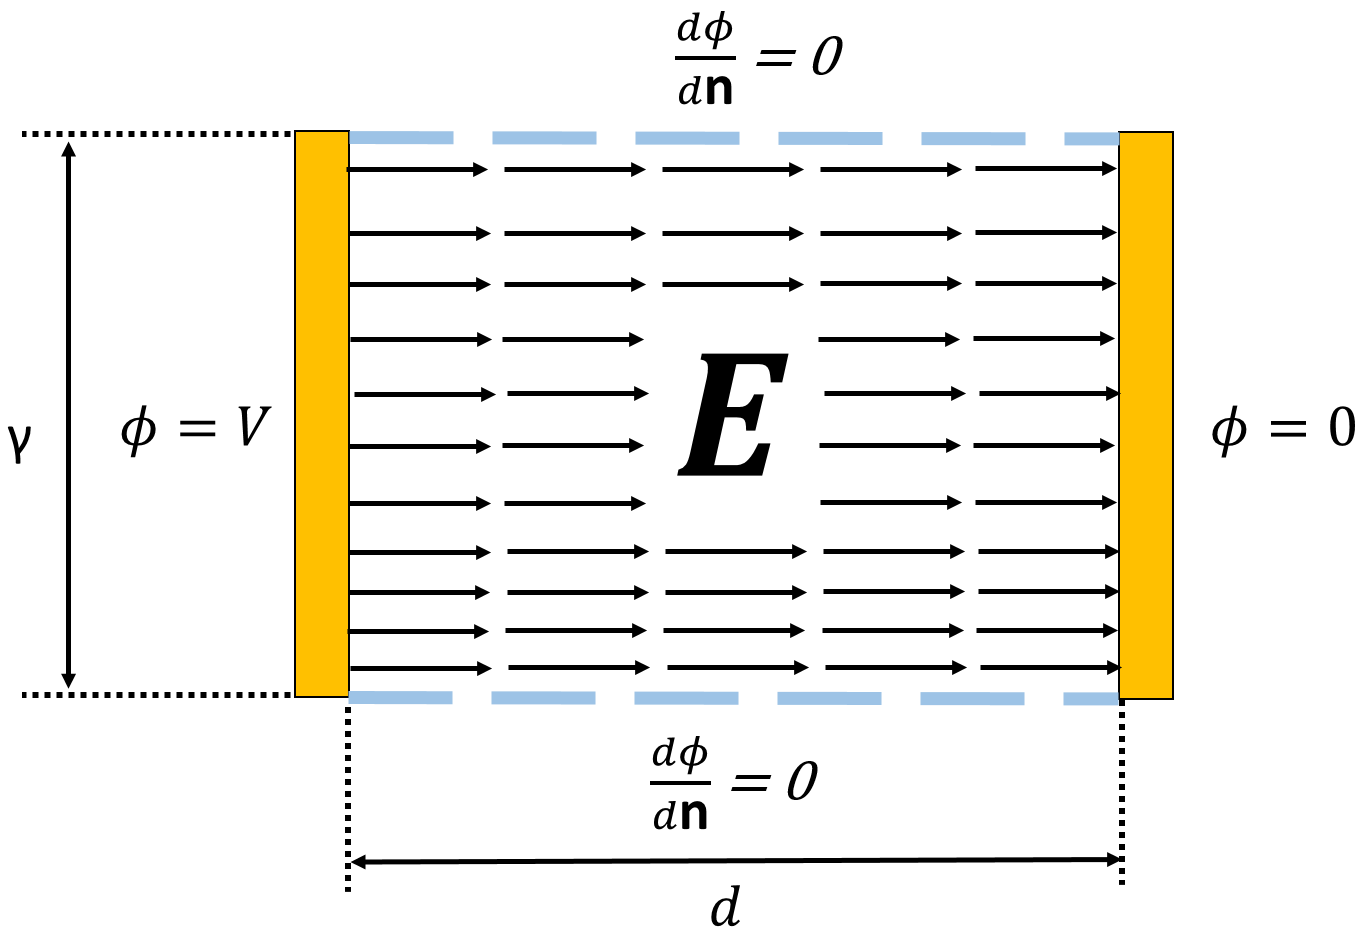
\includegraphics[width=0.7\textwidth]{images/capacitorNoFringe.png}
        \caption[Uniform electric field between parallel plates]{Uniform electric field between two parallel electrodes where $\boldsymbol{E}$ is the electric field, $\phi$ is the voltage, and $\frac{d\phi}{d\boldsymbol{n}}=0$ is the boundary condition of a perfect insulator. The dimensions of the capacitor are the electrode height $\gamma$, and the distance between the electrodes $d$.}
        \label{fig:parallelCapacitorModel}
  \end{figure}

    \par Sun, Greene, et al. utilized the Schwartz-Christoffel transform to map the coplanar electrode configuration in figure \ref{fig:simplified_IS_models} to the configuration of parallel electrodes with uniform electrode fields in figure \ref{fig:parallelCapacitorModel} \cite{sun_analytical_2007}. The Schwartz-Christoffel formula is a powerful transform that allows the mapping of the upper complex T-plane ($y>0$) to the inside of a polygon. The formula is
    
    \begin{equation}
        Z = C_1 \int_{T_0}^T \prod^m_{r=1} (T - T_r)^{(\theta_r/\pi - 1)} dT + C_2
    \end{equation}
    
    \noindent where $Z$ is the interior of a polygon in the Z-plane with vertices $Z_1,\;Z_2,\;Z_3,\; ...,Z_m$ and angles $\theta_1,\;\theta_2,\;\theta_3,\; ...,\theta_m$ which correspond to the points $T_1,\;T_2,\;T_3,\; ...,T_m$ on the real axis of the T-plane. $C_1$ and $C_2$ are integration constants. The Schwartz-Christoffel transform has three degrees of freedom, and consequently, up to three points may be chosen arbitrarily. $T_0$ is the reference and is typically chosen at the origin.
    
    \par A brief solution for the co-planar electrode system is covered in the following section with the complete step-by-step solution included in appendix \ref{app: complete_scm}.
    
    \par To find the geometric constant for coplanar electrodes, Schwartz-Christoffel transforms will be used to map half of the co-planar electrode geometry (Z-plane) to the upper complex plane (T-plane) and then to map the T-plane to half of the ideal parallel plate geometry. The W-plane vastly simplifies the solution to the cell constant and will allow the direct calculation of the ratio $\gamma$ to $d$. Figure \ref{fig:scm_planes_models} diagrams the three mapped planes. 
  \begin{figure}[h]
        \centering
        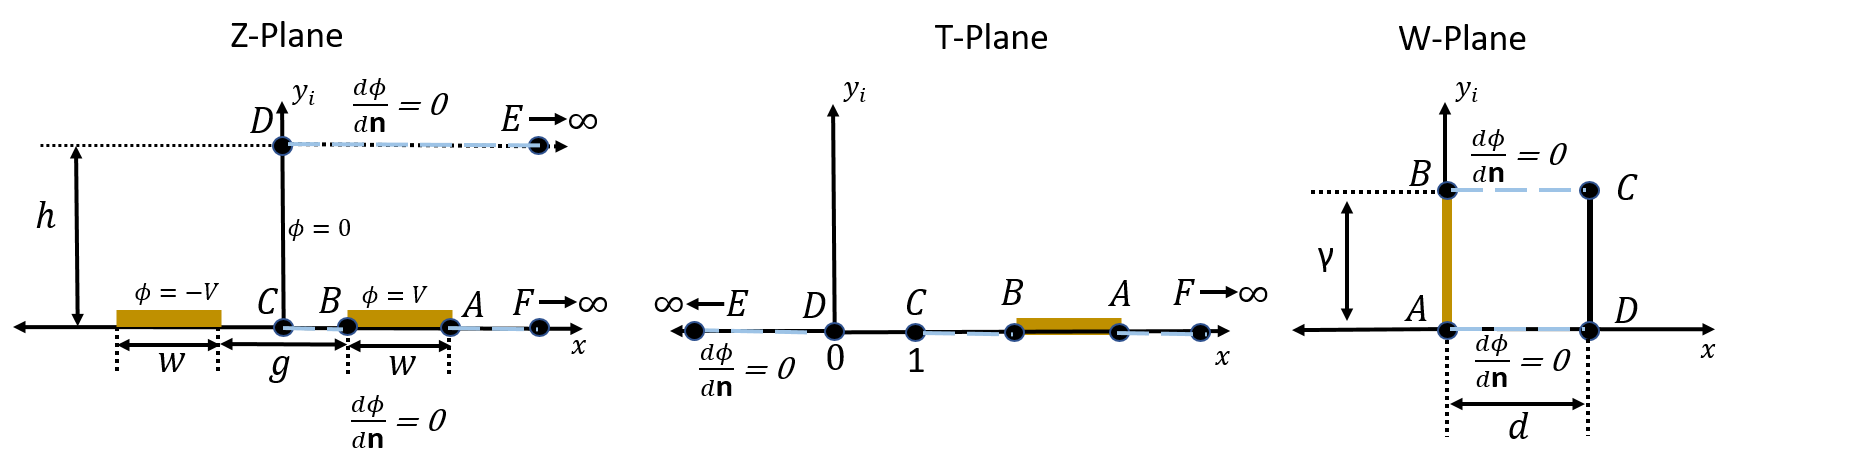
\includegraphics[width=\textwidth]{images/scmPlanes.png}
        \caption[Diagrams of coplanar electrodes through Schwartz-Christoffel mapping]{Diagrams of coplanar electrodes through Schwartz-Christoffel mapping where the Z-plane contains the physical dimensions of the electrode configuration, the T-Plane links the Schwartz-Christoffel mappins of Z and W plane, and the W-plane represents the parallel electrodes producing a uniform electrode field.}
        \label{fig:scm_planes_models}
    \end{figure}

\subsection*{Schwartz-Christoffel Transform Mapping}

  \par Mapping the T-plane to the Z-plane, point $C$ and $D$ from figure \ref{fig:scm_planes_models} will be chosen as the polygon corners with angles of $\pi/2$.  
   \begin{equation}
      Z = C_1\int (T-T_c)^{-1/2}(T-T_D)^{-1/2}dT + C_2
      \label{eqn:SCM_ZT_int}
  \end{equation}
  
 \noindent By integrating equation \ref{eqn:SCM_ZT_int} with the coordinate relationships $Z_C = 0$, $T_C = 1$ and $Z_D = jh$, $T_D = 1$, the mapping between the Z-plane and the T-plane can be expressed as
  
   \begin{equation}
     Z = \frac{2h}{\pi}\ln\Big(\sqrt{T-1} + \sqrt{T}\Big)
     \label{eqn:TZ}
 \end{equation}
 
 \noindent The mapping of the T-plane to the Z-plane is depicted in figure \ref{fig:T_to_Z_mapping}. 
 
    \begin{figure}[h]
    \centering
    \begin{subfigure}[t]{0.45\textwidth}
        \centering
        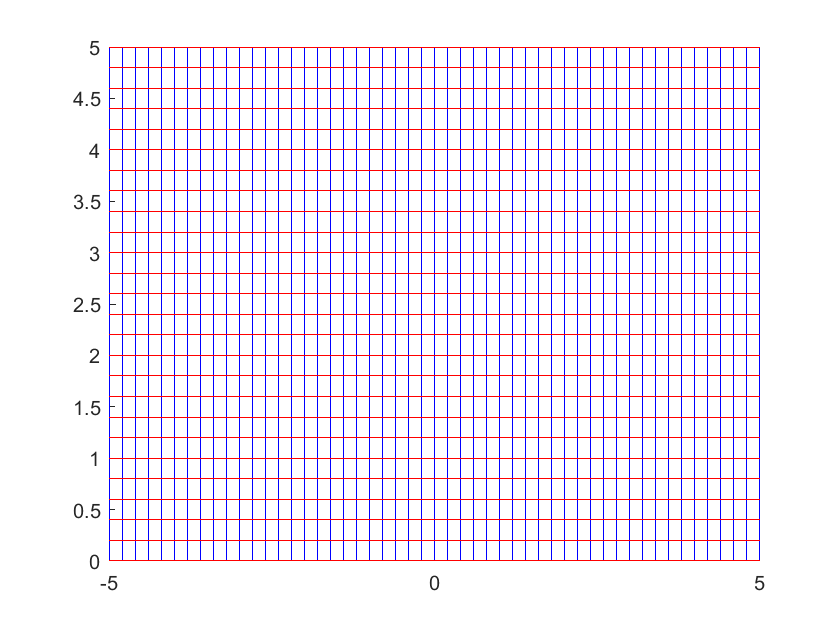
\includegraphics[width=\textwidth]{images/TtoZ_strip.png}
        \caption{Part of upper complex T-Plane}
    \end{subfigure}
    \hfill
    \begin{subfigure}[t]{0.45\textwidth}
        \centering
        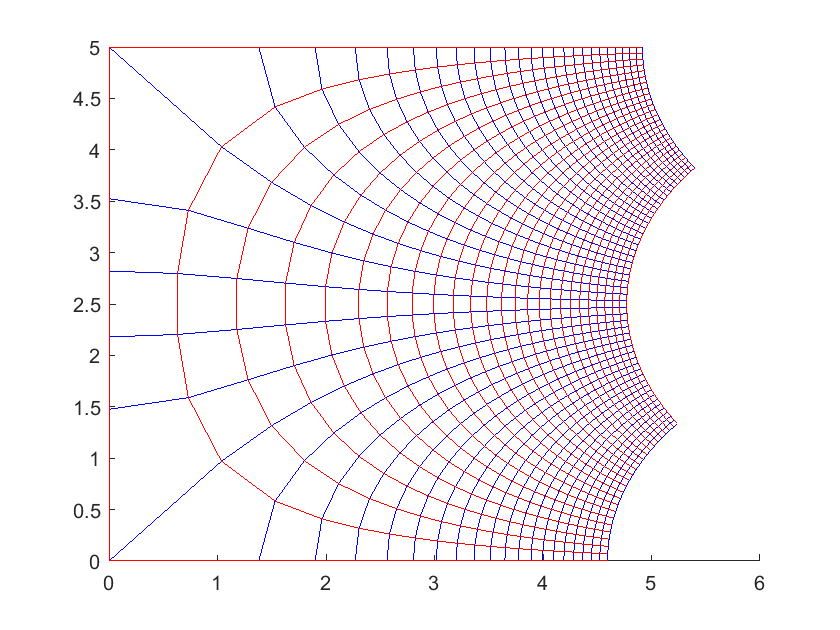
\includegraphics[width=\textwidth]{images/TtoZ_map.png}
        \caption{Mapping of the part of the T-plane to the polygon in the Z-plane}
    \end{subfigure} 
    \caption[Mapping of the T-plane to the inside of the open polygon in the Z-Plane]{Mapping of the T-plane to the inside of the open polygon in the Z-Plane outlined by the points $F$, $C$, $D$, and $E$ in the Z-plane. Equation \ref{eqn:TZ} is the mapping function.} 
    \label{fig:T_to_Z_mapping}
 \end{figure}

\par The mapping of the Z-plane to the T-plane can be found by solving for the inverse of equation \ref{eqn:TZ}.

\begin{equation}
     T = \cosh^2\bigg(\frac{z\pi}{2h}\bigg)
     \label{eqn:ZT}
 \end{equation}

\noindent Figure \ref{fig:Z_to_T_mapping} depicts the mapping of the Z-plane to the T-plane.

     \begin{figure}[h]
    \centering
    \begin{subfigure}[t]{0.45\textwidth}
        \centering
        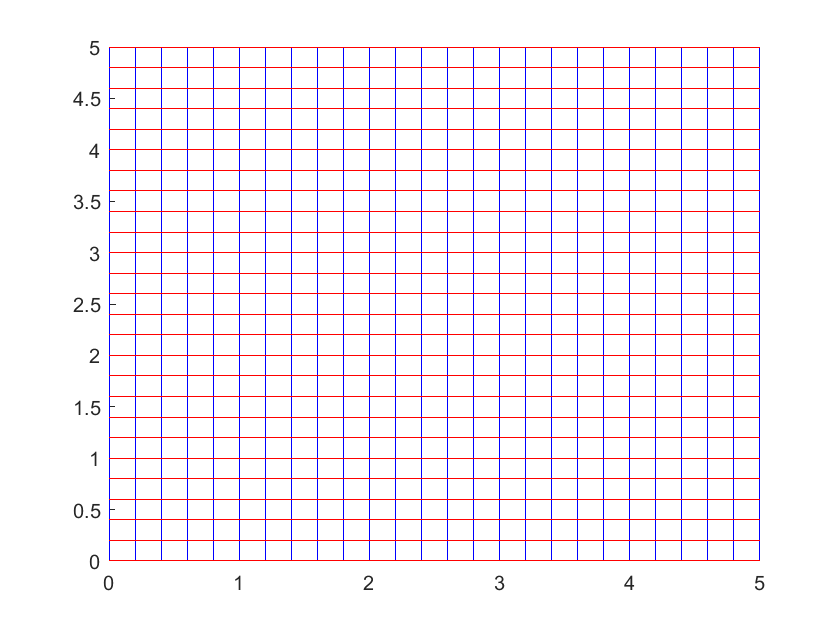
\includegraphics[width=\textwidth]{images/ZtoT_strip.png}
        \caption{Part of the open polygon in the Z-plane.}
    \end{subfigure}
    \hfill
    \begin{subfigure}[t]{0.45\textwidth}
        \centering
        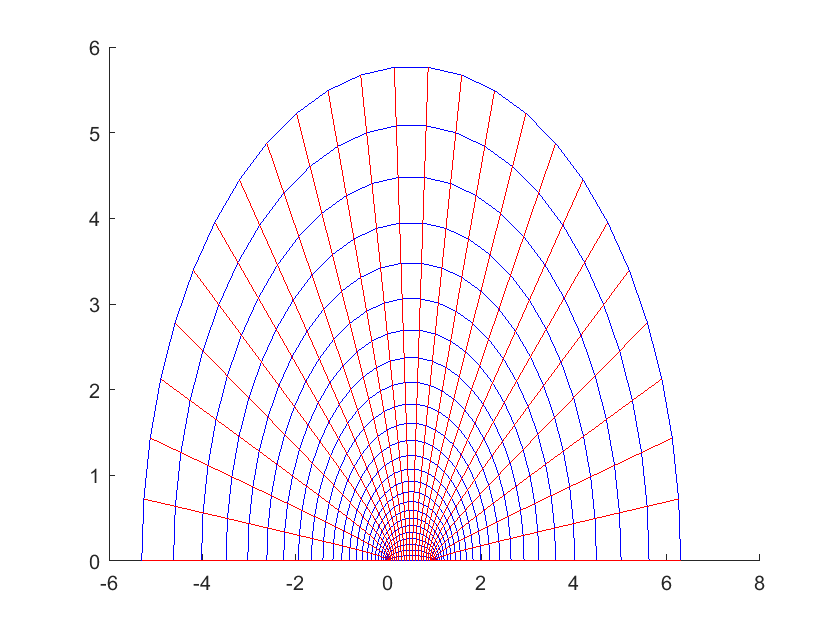
\includegraphics[width=\textwidth]{images/ZtoT_map.png}
        \caption{Mapping of part of the polygon in the Z-plane to the T-plane.}
    \end{subfigure} 
    \caption[Mapping of the open polygon in the Z-Plane to the T-plane.]{Mapping of the open polygon in the Z-Plane outlined by the points $F$, $C$, $D$, and $E$ to the T-plane. Equation \ref{eqn:ZT} is the mapping function.} 
    \label{fig:Z_to_T_mapping}
 \end{figure}

 \par Mapping the T-plane to the W-Plane, points $A$, $B$, $C$, and $D$, will be chosen as the polygon corners with angles of $\pi/2$.
 \begin{equation}
    W = D_1 \int (T-T_A)^{-1/2}(T-T_B)^{-1/2}(T-T_C)^{-1/2}(T-T_D)^{-1/2}\;dT + D_2
    \label{eqn:scm_wt_int}
 \end{equation}
 
 \noindent Since equation \ref{eqn:scm_wt_int} is an integral of a rational function with a root of a quartic polynomial, the function can be rewritten as an elliptic integral \cite{i.s._gradshteyn_table_1980}.
 
 \begin{equation}
     W = D_3F(v,k) + D_2
 \end{equation}
 \begin{equation}
    D_3 = \frac{2D_1}{\sqrt{(T_A - T_C)(T_B-T_D)}}
 \end{equation}
 
 \begin{equation}
     v = \arcsin\sqrt{\frac{(T_B-T_D)(T-T_A)}{(T_A-T_D)(T-T_B)}}
 \end{equation}
 
 \begin{equation}
     k = \sqrt{\frac{(T_B-T_C)(T_A-T_D)}{(T_A-T_C)(T_B-T_D)}}
 \end{equation}
 \noindent Where $F(v,k)$ is the incomplete elliptic integral of the first kind, and can be expressed as
 \begin{equation}
     F(v,k) = \int^v_0 \frac{d\alpha}{\sqrt{1 - k^2\sin^2\alpha}}
 \end{equation}
 \noindent Where $v$ and $k$ are referred to as the amplitude and modulus respectively.
 
 \par Using the coordinate relations for point A: $W_A = 0$, $F\big(v(T_A),k\big) = 0$; point B: $W_B = j\gamma$, $F\big(v(T_B +\lim_{x\to 0} jx),k\big) = jK(k')$; and point D: $W_D = d$, $F\big(v(T_D),k\big) = K(k)$; we find that 
 
 \begin{equation}
     D_2 = 0,
 \end{equation}
 \begin{equation}
     D_3 = \frac{d}{K(k)},
     \label{eqn:D3 w/ d}
 \end{equation}
\noindent and
\begin{equation}
    D_3 = \frac{j\gamma}{K(k')}.
    \label{eqn:D3 w/ gamma}
\end{equation}

\noindent Where $K(k)$ is the complete elliptic integral and is expressed as 

 \begin{equation}
     K(k) = \int_0^{\pi/2} \frac{d\alpha}{1 - k^2\sin^2(\alpha)}
 \end{equation}
 
 \noindent and where $k'$ is the complement modulus and is expressed as 
 \begin{equation}
     k' = \sqrt{1-k^2}
 \end{equation}

\noindent By combining equations \ref{eqn:D3 w/ d} and \ref{eqn:D3 w/ gamma} we get

\begin{equation}
    \frac{\gamma}{d} = \frac{K(k')}{K(k)}
    \label{eqn:d gamma relationship}
\end{equation}

\noindent and then substituting equation \ref{eqn:d gamma relationship} into equation \ref{eqn: cellConstants}, we find that the cell constant and geometric factor for co-planar electrodes are 

\begin{equation}
    \kappa = \frac{2K(k)}{lK(k')}
    \label{eqn: cellConstantSolution}
\end{equation}

\begin{equation}
    G_f = \frac{lK(k')}{2K(k)}
\end{equation}

\par It should be noted that the current mapping of the T-plane to W-plane is unconstrained with no solution to the constant $D_3$. By selecting a value for either $D_3$, $\gamma$, or $d$, we constrain the mapping, but the actual value we choose is of no consequence to the electrical behaviour of the system. Physically, this is explained since the cell constant is defined by the ratio of $d$ and $\gamma$ and, given the same material properties, as long the ratio in equation \ref{eqn:d gamma relationship} is maintained, the effective impedance will be the same. There are an infinite number of W-planes that satisfy the ratio in equation \ref{eqn:d gamma relationship}. For mapping the T-plane to the W-plane, $D_3$ can be arbitrarily chosen. If $D_3$ is chosen to be 1, the W transform can be expressed as 

\begin{equation}
    W = F(v,k).
    \label{eqn: w_mapping}
\end{equation}

\noindent Figure \ref{fig:Z_to_w_mapping} depicts the mapping the T-plane to the W-plane. 

\begin{figure}[h]
    \centering
    \begin{subfigure}[t]{0.45\textwidth}
        \centering
        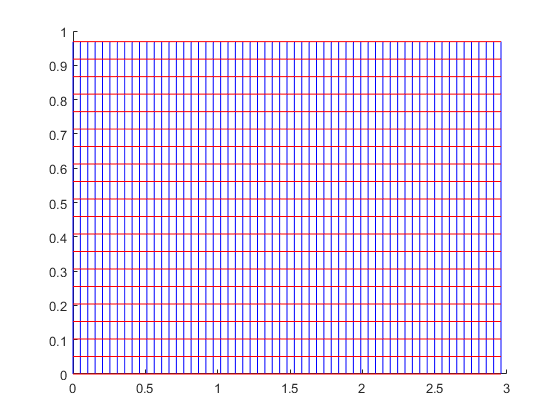
\includegraphics[width=\textwidth]{images/z2w_zplane.png}
        \caption{Part of the open polygon in the Z-plane.}
    \end{subfigure}
    \hfill
    \begin{subfigure}[t]{0.45\textwidth}
        \centering
        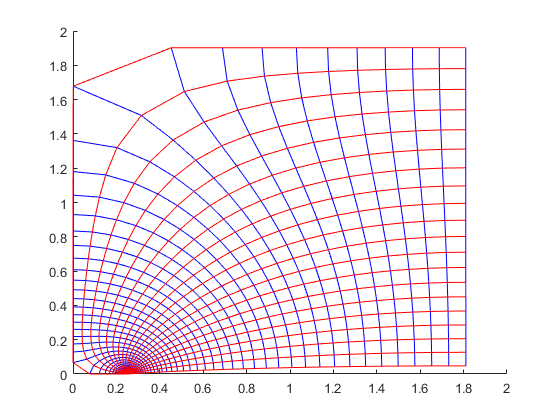
\includegraphics[width=\textwidth]{images/z2w_w-plane.png}
        \caption{Mapping of part of the polygon in the Z-plane to the W-plane.}
    \end{subfigure} 
    \caption[Mapping of the open polygon in the Z-Plane to the W-plane.]{Mapping of the open polygon in the Z-Plane outlined by the points $F$, $C$, $D$, and $E$ to the W-plane. Equation \ref{eqn: w_mapping} is the mapping function.} 
    \label{fig:Z_to_w_mapping}
 \end{figure}

\subsection{Coplanar Electric Field}

 \par With Z-T and T-W mappings, the solution of the electric field in the W-plane can be mapped to the Z-plane. The mapping of the electric field can be expressed as 
 
 \begin{equation}
     \boldsymbol{E_z} = -\nabla \phi_z \;\;\text{with} \;\;\;\nabla \phi_z = \nabla \phi_w \overline{\frac{dW}{dZ}}
     \label{eqn:ZtoW_efield}
 \end{equation}
 
 \noindent Where $\nabla \phi$ is the gradient of potential and $\overline{\frac{dW}{dZ}}$ is the conjugate of the derivative of $W$ with respect to $Z$ \cite{schinzinger_conformal_2012}.
 
 \par Applying the chain rule to equation \ref{eqn:ZtoW_efield}, the electric field mapping is expressed as
 \begin{equation}
    \boldsymbol{E_z} =- \nabla \phi_w \overline{\frac{dW}{dT}\frac{dT}{dZ}}
    \label{eqn:ZtoW_efield_chain}
 \end{equation}
\noindent with 
 \begin{equation}
     -\nabla \phi_w = \frac{V}{d},
     \label{eqn:phi_w}
 \end{equation}
 \begin{equation}
     \frac{dW}{dT} = \frac{d}{2K(k)}\frac{(T_A - T_C)^{1/2}(T_B-T_D)^{1/2}}{(T-T_A)^{1/2}(T-T_B)^{1/2}(T-T_C)^{1/2}(T-T_D)^{1/2}},
     \label{eqn:dwdt}
 \end{equation}
 \noindent and
 \begin{equation}
     \frac{dT}{dZ} = \frac{\pi}{h}(\sqrt{T-T_D})(\sqrt{T-T_C}).
     \label{eqn:dtdz}
 \end{equation}
 
 \par Combining equations, \ref{eqn:ZtoW_efield_chain}, \ref{eqn:phi_w}, \ref{eqn:dwdt}, and \ref{eqn:dtdz}, the electric field for the co-planar electrodes can be expressed as equation \ref{eqn:Ez} and is depicted with streamlines in figure \ref{fig:electricFieldStreamLines} and as electric field magnitude in figure \ref{fig:electricFieldMag}. A complete step-by-step solution is provided in appendix \ref{app: complete_scm}.
 
 \begin{equation}
    E_z = \overline{\frac{\pi V}{2hK(k)} \frac{\sqrt{(T_A-T_C)(T_B-T_D)}}{\sqrt{(T-T_A)(T-T_B)}}}
    \label{eqn:Ez}
 \end{equation}
 
    
     \begin{figure}[h]
    \centering
    \begin{subfigure}[b]{\textwidth}
        \centering
        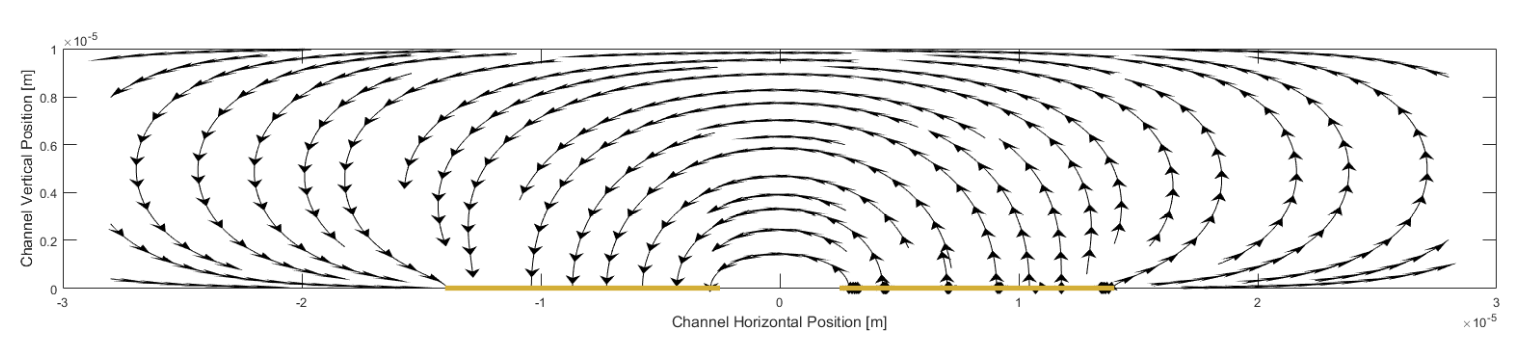
\includegraphics[width=\textwidth]{images/electricFieldStreamLines.png}
        \caption{Electric field stream lines for co-planar electrodes.}
        \label{fig:electricFieldStreamLines}
    \end{subfigure}
    \\
    \vspace{0.2 in}
    \begin{subfigure}[b]{\textwidth}
        \centering
        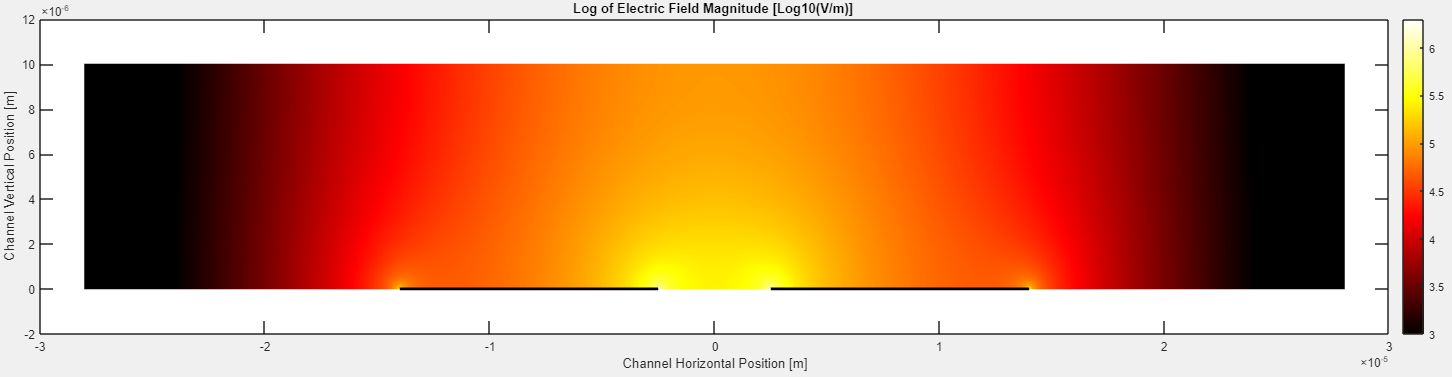
\includegraphics[width=\textwidth]{images/EfieldMagnitude.png}
        \caption{Electric field magnitude generated by co-planar electrodes. The magnitude is reported in units Log$_{10}$(V/m).}
        \label{fig:electricFieldMag}
    \end{subfigure} 
    \caption[Electric Field of Co-planar Electrodes]{The electric field for co-planar electrodes as defined by equation \ref{eqn:Ez} . The electrodes are 11.5 $\mu$m wide with a 5 $\mu$m gap and the chamber is 10 $\mu$m tall.}
    \label{fig:electricFieldPlots}
 \end{figure}

\newpage

\subsection{Novel Volume Fraction}
\par The traditional method to approximate the volume fraction of a single spherical particle suspended over co-planar electrodes is to take the ratio of the cell volume divided by the volume of the electrodes in the channel.

\begin{equation}
    \phi = \frac{\frac{4}{3}\pi R^3}{(2w+g)hl}
\end{equation}

\noindent where $R$ is the particle radius, $w$ is the electrode width, $d$ is the gap between the coplanar electrodes, $h$ is the height of the channel, and $l$ is the length of the electrodes in the channel. This approximation assumes that the fringe fields outside the boundaries of the electrodes is negligible and that the electric field magnitude is uniform inside the boundaries of the electrodes. However, for most co-planar electrode geometries used in impedance spectroscopy, the electric field is highly non-uniform. Figure \ref{fig:electricFieldPlots} depicts the non-uniformity of an electric field produced by co-planar electrodes. In this section, I propose two alternative approaches to calculating the correct volume fraction. 

\subsection*{Mapping Particle Volume to the W-Plane}
\par To calculate the effective volume fraction it is necessary to calculate the ratio of effective volumes:

\begin{equation}
    \phi ' = \frac{V_p'}{V_{sys}'},
\end{equation}
\noindent where $\phi '$ and $V '$ denotes the effective volume fraction and volume respectively. By examining a particle suspended in the Z-plane it is difficult to determine the what the effective volume for the system or the particle is due to the non-uniform electric fields. However, the electric field is uniform when the system is mapped to the w-plane. The effective volume fraction can be expressed as 
\begin{equation}
    \phi ' = \frac{V^w_p}{V^w_{sys}}
\end{equation}
\noindent where $w$ denotes volumes in the w-plane.

\par By referring to the ideal capacitor geometry in figure \ref{fig:parallelCapacitorModel}, the system volume in the w-plane can be expressed as 
\begin{equation}
    V^w_{sys} = \gamma d l,    
\end{equation}
\noindent and by substituting in equations \ref{eqn:D3 w/ d} and \ref{eqn:D3 w/ gamma}, and remembering $D_3$ was arbitrarily chosen as 1 for the W-mapping, we find

\begin{equation}
    V^w_{sys} = 2K(k)K(k')l.
    \label{eqn: Vwsys}
\end{equation}

\par When a spherical particle is mapped to the W-plane, the particle cross-sections are deformed based on the non-uniformity of the electric field. If we assume that these cross-sections are deformed to either "circle-like" or "ellipsoid-like" sections, the mapped volume of the sphere can be approximated as 

\begin{equation}
    V^w_p = \frac{4}{3}\pi r_z r_{w1} r_{w2},
    \label{eqn:Vwp radii}
\end{equation}

\noindent where $r_z$ is the radius of the spherical particle in the z-plane, and $r_{w1}$ and $r_{w2}$ are the principle radii of the "ellipsoid-like" mapping of the particle orthodrome to the w-plane. Equation \ref{eqn:Vwp radii} can be rewritten as 

\begin{equation}
    V^w_p = \frac{4}{3} r_z \iint_{A_w} dA,
    \label{eqn: Vwp}
\end{equation}

\noindent where the integral represents the area of the particle orthodrome mapped to the w-plane. 

\par Combining equations equations \ref{eqn: Vwsys} and \ref{eqn: Vwp}, we can approximate the effective volume fraction as
\begin{equation}
    \phi_w = \frac{2}{3} \frac{r_z \iint_{A_w} dA}{K(k)K(k'))l}
\end{equation}

\par The major shortcoming of this method is operating under the assumption that the mapped particle cross-sections are circle or ellipsoid-like. From empirical tests, many particle-electrode configurations result in particle cross-sections that do appear circular or ellipse-like, but there will be an associated error that will often grow with the degree of the non-uniformity. Compared to the traditional volume fraction, the error is minimal. The w-plane volume fraction accounts for fringe field effects and the local non-uniformity of the electric field, allowing for the calculation of the volume fraction for a particle located anywhere in the system. 

\subsection*{Power Volume Fraction}
\par In the w-plane, which represents the ideal parallel plate electrode model depicted in figure \ref{fig:parallelCapacitorModel}, the electric field is uniform inside the valid domain and as a direct result, the power density is uniform thought the domain of the w-plane. By recognizing that the effective volume fraction is the ratio of volumes in the w-plane, we arrive at the following relationship:
\begin{equation}
    \phi ' = \frac{V_p'}{V_{sys}'} = \frac{V^w_p}{V^w_{sys}} = \frac{P_p}{P_{sys}}.
    \label{eqn: effectiveVolumeFractions}
\end{equation}

\par By finding the ratio of power in the domain of the particle to the power of the system, we are able to calculate the effective volume fraction as the power fraction:
\begin{equation}
    \phi_p = \frac{P_p}{P_{sys}},
    \label{eqn: powerVolumeFraction_initial}
\end{equation}

\par The power the system can be expressed as
\begin{equation}
    P_{sys} = \frac{(2V)^2}{R_{sys}},
\end{equation}
\noindent and by recalling that $R=\rho\kappa$,
\begin{equation}
    P_{sys} = \frac{4V^2}{\rho\kappa}.
\end{equation}
\noindent By substituting equation \ref{eqn: cellConstantSolution}, for the cell constant, the power of the system is expressed as 
\begin{equation}
    P_{sys} = \frac{2V^2K(k')l}{\rho K(k)}
    \label{eqn: powerSystem}
\end{equation}

\par The power in the region of a spherical particle can be solved for by integrating the power density over the volume of the particle.
\begin{equation}
    P_p = \iiint_V \rho \big| J \big| dV = \iiint_V \frac{1}{\rho} \big| E \big|^2 dV
\end{equation}
\noindent And then by substituting the solution of the electric field from equation \ref{eqn:Ez}, we can express the power in the domain of the particle as
\begin{equation}
    P_p = \frac{1}{\rho}\bigg(\frac{\pi^2 V^2}{4h^2K(k)^2}\bigg)\iiint_V \bigg|\bigg(\frac{T_A-T_C}{T-T_A}\bigg)\bigg(\frac{T_B-T_D}{T-T_B}\bigg)\bigg| \;dV
    \label{eqn: powerParticle}
\end{equation}

Combining equations \ref{eqn: powerVolumeFraction_initial}, \ref{eqn: powerSystem}, and \ref{eqn: powerSystem}, the power fraction can be expressed as
\begin{equation}
    \phi_p = \frac{\pi^2 K(k)}{8h^2K(k)K(k')l}\iiint_V \bigg|\bigg(\frac{T_A-T_C}{T-T_A}\bigg)\bigg(\frac{T_B-T_D}{T-T_B}\bigg)\bigg| \;dV
\end{equation}

\par If the particle is a sphere, the integral can conveniently be expressed in spherical coordinates:
\begin{equation}
    \phi_p(Z_c,R) = 2C\int_{0}^\frac{pi}{2}\int_0^{2\pi}\int_0^R r^2 \sin(\phi)F(r,\theta,\phi,Z_c)dr\,d\theta\,d\phi,
\end{equation}
\noindent where $Z_c$ is the center of the particle, R is the radius,
\begin{equation}
    F(r,\theta,\phi) = \bigg|\bigg(\frac{T_A-T_C}{T(r,\theta,\phi,Z_c)-T_A}\bigg)\bigg(\frac{T_B-T_D}{T(r,\theta,\phi,Z_c)-T_B}\bigg)\bigg|,
\end{equation}
\begin{equation}
    T(r,\theta,\phi,Z_c) = \cosh^2\bigg(\frac{\pi}{2h}\Big(Z_c+r\cos(\frac{\pi}{2}-\phi)e^{i\theta}\Big)\bigg),
\end{equation}
\noindent and
\begin{equation}
    C = \frac{\pi^2}{8h^2K(k)K(k')l}.
\end{equation}

\par The power fraction provides an exact solution to the volume fraction for the co-planar electrode system outlined in section \ref{sec: coplanarElectrodeCellConstant}. These corrected volume fractions allow for a complete analytic impedance solution that accounts for the effect of the fringe field and non-uniform electric field based on the position of the particle. If incorporated in a drag-flow model, flow-through IS systems can be simulated with respect to time.


\subsection{Device Sensitivity}
\par Linderholtz defined the sensitivity of a device as the local dissipation of power normalized by the total power of the system. In otherwords, Linderholtz sensitivity is the ratio of power density at a point in the system to the power of the system and can be expressed as

\begin{equation}
    S_{Linderholtz} = \frac{\rho |j|^2}{R_{sys}V_{sys}^2}.
    \label{eqn:Linderholtz}
\end{equation}

\noindent The Linderholtz definition of sensitivity takes into account the non-uniformity of of the electric field, but does not include the dielectric properties of the particle and the medium.

\par Sun proposed an alternative sensitivity definition as the ratio or relative impedance to the impedance of the medium.

\begin{equation}
    S_{Sun} = \frac{| |\Tilde{Z}_{mix}| - |\Tilde{Z}_m| |}{|\Tilde{Z}_m|}
\end{equation}

\par Sun's definition has the advantage of taking into account the the dielectric properties of the suspension. In contrast to Linderholtz sensitivity, Sun determined that there was no optimal electrode geometry but is rather the maximization of the volume fraction. However, his calculations used the standard method of determining the volume fraction, which does not account for non-uniformity of the electric field local to the position of the particle. 

\par By using the power volume fraction with Sun's definition of sensitivity, we get the advantages of both sensitivity definitions: the ability to account for dielectric properties and local non-uniformity in the power density over the region of the particle.

\subsection{Analytic Impedance Modeling Tool}

\par The analytic impedance solution for co-planar electrode systems was implemented in the MATLAB programming language. The code for the simulations is provided in the appendix \ref{app: IS_code}. To facilitate simulation and exploration of the analytice impedance solution, the MATLAB application, the IS App, was created. The IS App collated the analytic impedance solution into a single program with a graphical user interface. The main page of the application is displayed in figure \ref{fig:matlab_IS_app}. The IS App is split into three sections: impedance spectroscopy, equivalent circuit values, and the electric field and volume fraction analysis. 

\begin{figure}[h]
    \centering
    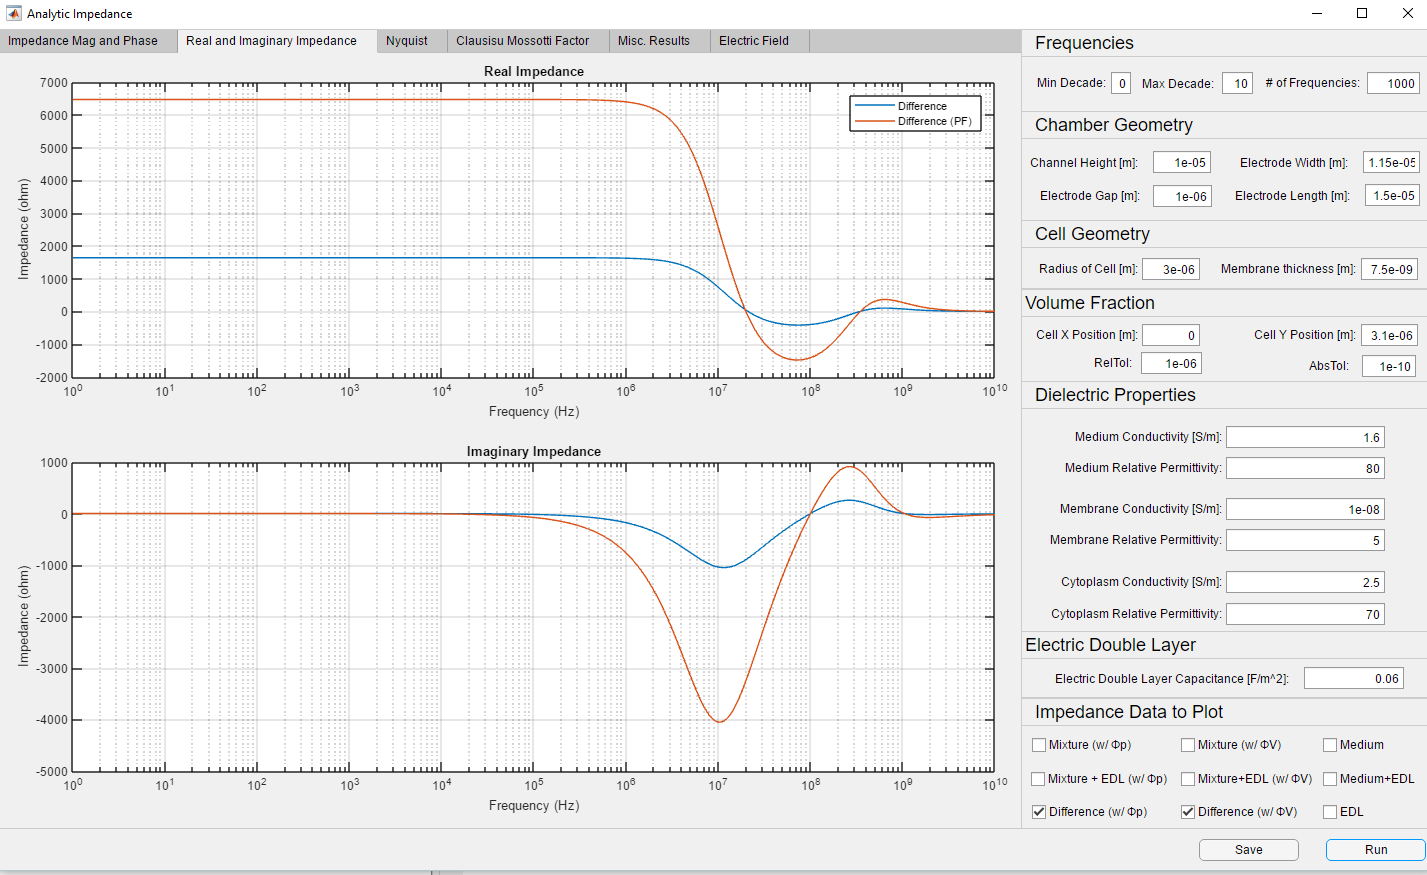
\includegraphics[width=\textwidth]{images/analyticImpedanceApp.png}
    \caption[IS App]{The IS app GUI created in MATLAB to calculate and display the analytic impedance solution to a single cell suspension over co-planar electrodes. The impedance is displayed as magnitude-phase, real-imaginary, and Nyquist plots. The IS app also includes the capability to calculate the Clausius Mossotti spectrum, an equivalent circuit model, the electric field of the co-planar electrode system, and a mapping of the cell orthodrome to the W-plane.}
    \label{fig:matlab_IS_app}
\end{figure}

\subsection*{Impedance Spectroscopy}

\par The main section of the IS App is the impedance spectroscopy simulation. The parameter entry section is located on the right side of the user interface depicted in figure \ref{fig:matlab_IS_app} and allows the user to dictate the parameters in the analytic impedance solution. It is important to keep in mind that the analytic impedance solution assumes that the channel length continues infinitely, but the electrode geometry, channel height, and particle geometry can all be specified. 

\par The parameters \textit{RelTol} and \textit{AbsTol} under the \textit{Volume Fraction} subsection affect the acceptable error tolerance when calculating the power volume fraction. Smaller values will provide more accurate answers at the expense of computing time. In most cases, the default values are more than sufficient. The current application requires so little computing time that there is little reason to increase the tolerance parameters from their default value, and few applications would require higher precision than currently provided.

\par The electric double layer capacitance parameter determines the effect of the EDL on the model. The model takes the simplest approach to the EDL and represents its as two capacitors in series to the analytic impedance solution. The capacitance is calculated by finding the product of the entered parameter and with the area of the electrodes. Implementation of the sophisticated EDL models should be considered for further development of the IS App. 

\par The checkmarks under the \textit{Impedance Data to Plot} subsection dictates what data sets will be plotted and saved after running the simulation. The \textit{mixture}, \textit{medium}, and \textit{difference} option denote the impedance solution of the single cell suspension, no-cell solution, and the difference between the single cell suspension and the no-cell solution impedance respectively. The \textit{EDL}, $\phi$V, and $\phi$p options calculates the analytic impedance solution with the electric double layer, the traditional volume fraction, and the power fraction respectively.

\begin{figure}[h]
    \centering
    \begin{subfigure}[b]{0.45\textwidth}
        \centering
        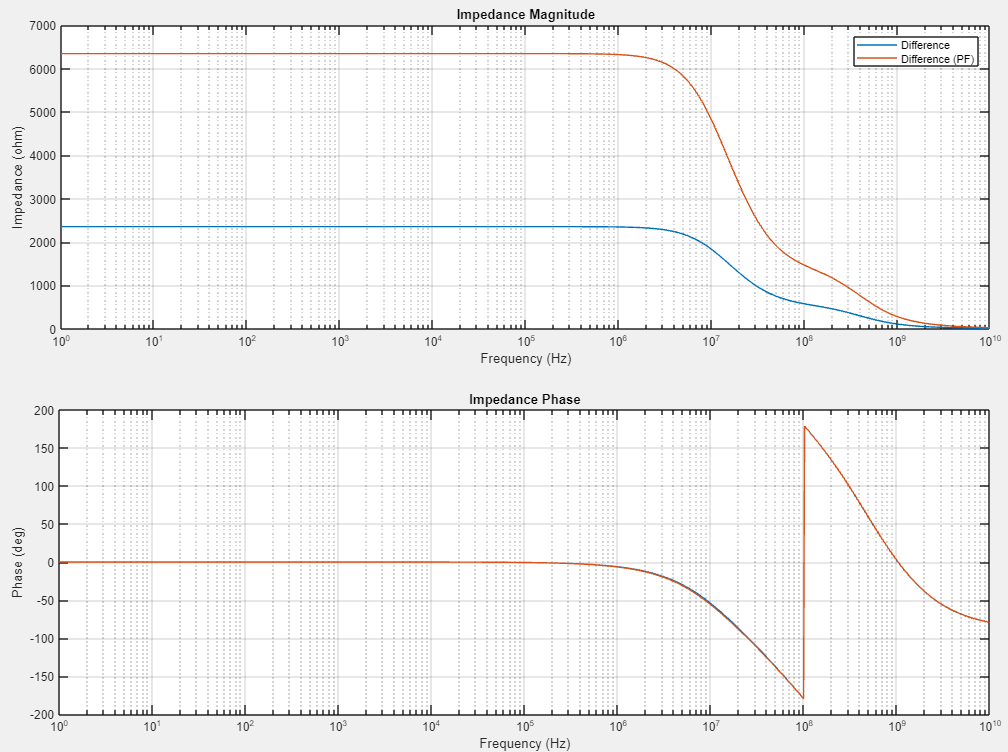
\includegraphics[width=\textwidth]{images/IS_APP_mag_phase.png}
        \caption{Impedance magnitude and phase}
    \end{subfigure}
    \hfill
    \begin{subfigure}[b]{0.45\textwidth}
        \centering
        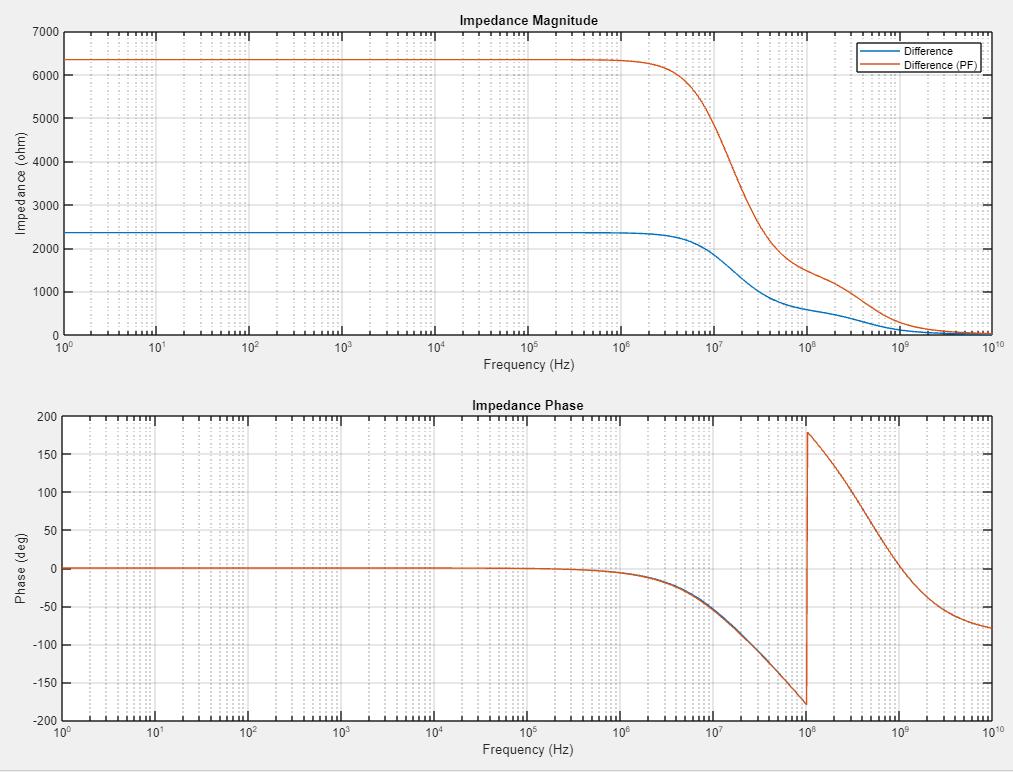
\includegraphics[width=\textwidth]{images/IS_APP_real_imag.png}
        \caption{Real and imaginary impedance}
    \end{subfigure}
    \\
    \vspace{0.1 in}
    \begin{subfigure}[b]{0.45\textwidth}
        \centering
        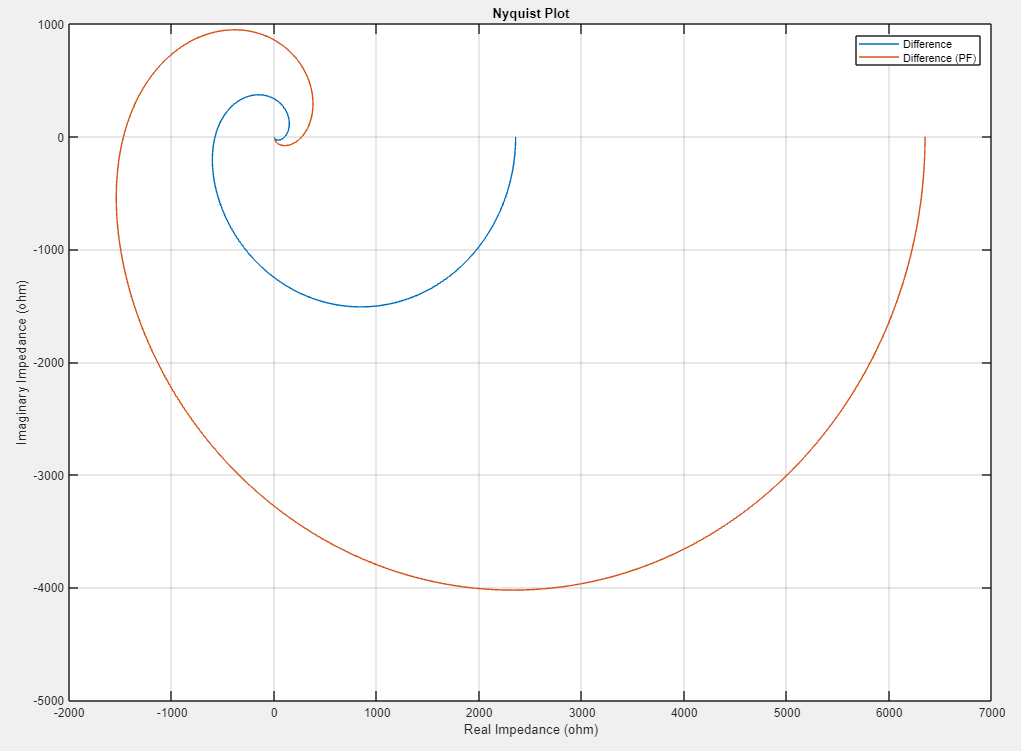
\includegraphics[width=\textwidth]{images/IS_APP_Nyquist.png}d
        \caption{Nyquist plot}
    \end{subfigure}
    \hfill
    \begin{subfigure}[b]{0.45\textwidth}
        \centering
        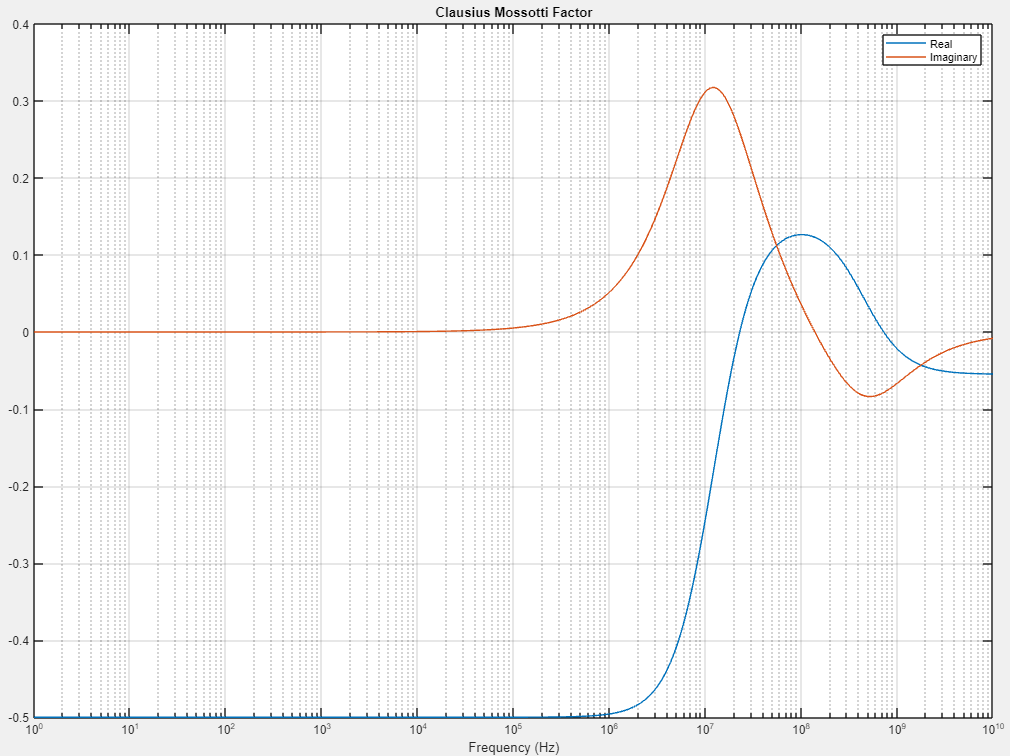
\includegraphics[width=\textwidth]{images/IS_APP_FCM.png}
        \caption{Clausius Mossotti Factor}
    \end{subfigure}
    \caption{Example plots depicting results of the analytic impedance solution generated by the IS App.}
    \label{fig:IS_APP_IS_Results}
\end{figure}

\par The IS App visualizes the results as impedance magnitude-phase plots, real-imaginary parts, a Nyquist plot, and the real and imaginary parts of the Clausius Mossotti factor. An example of the plots is given in figure \ref{fig:IS_APP_IS_Results}.

\subsection*{Equivalent Circuit}
\par The equivalent circuit section of the the IS App uses the Foster-Schwan model to calculate the equivalent circuit values for the single cell suspension described by the parameter entries displayed in figure \ref{fig:matlab_IS_app}. A full explanation of the Foster-Schwan model is provided in section \ref{sec: cell_suspension_equiv_circ}. The equivalent circuit section of the IS App is displayed in figure \ref{fig:is_app_equivalent_circuit}. For comparison purposes, the equivalent circuit values using both the traditional fraction and the power fraction are provided.

\begin{figure}[h]
    \centering
    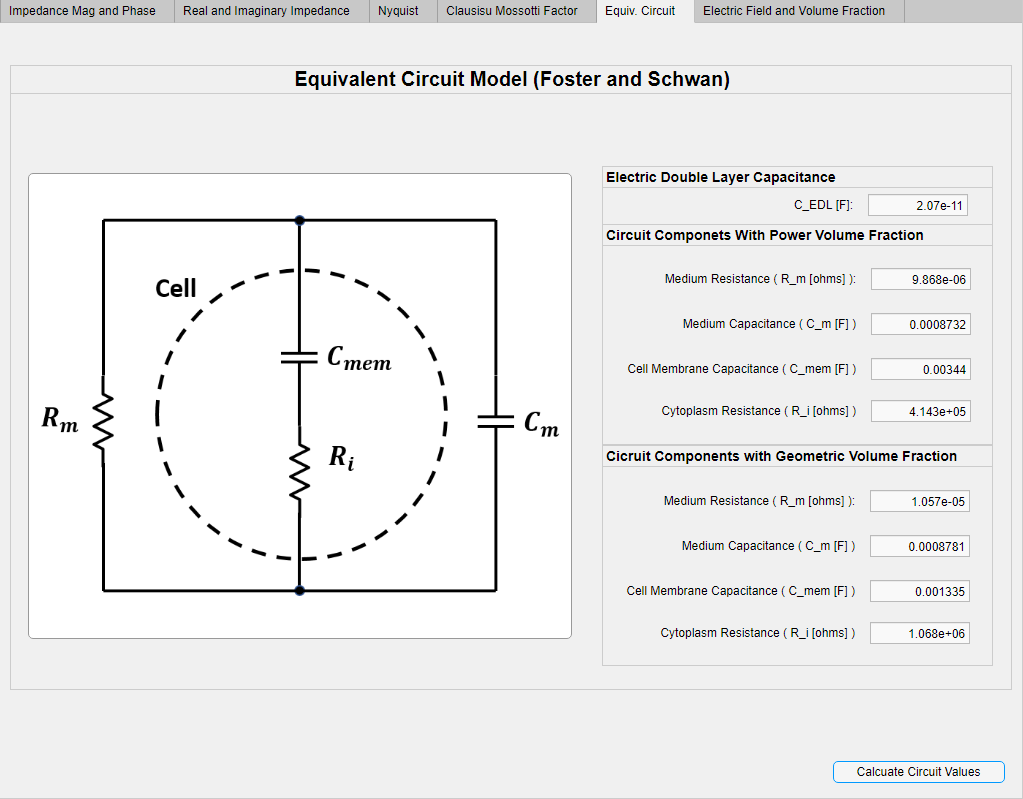
\includegraphics[width=\textwidth]{images/impedanceDisplayEquivCircuitV2.png}
    \caption{The IS app display for the equivalent circuit model of a single cell suspension.}
    \label{fig:is_app_equivalent_circuit}
\end{figure}

\subsection*{Electric Field and Volume Fraction}

\par The electric field and volume fraction section of the IS App was created to depict how the geometry of the system affects the electric field and volume fraction. The electric field and volume fraction section of the program is displayed in figure \ref{fig:is_app_Efield_volume_fraction}. 

\begin{figure}[h]
    \centering
    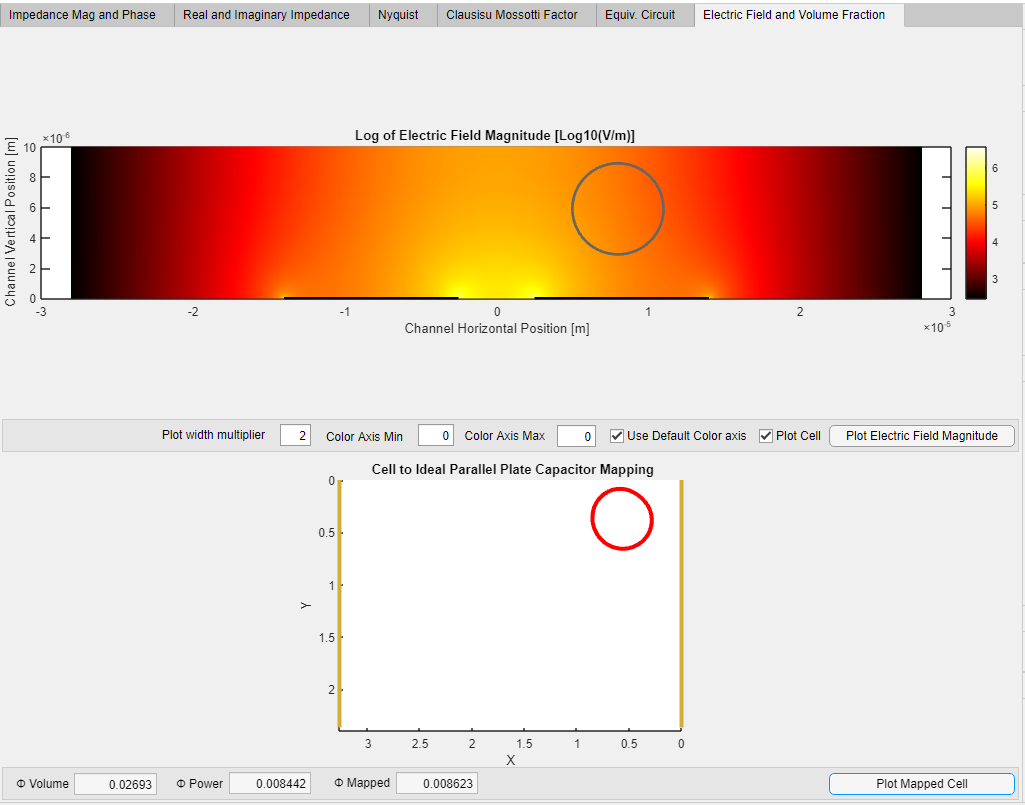
\includegraphics[width=\textwidth]{images/impedanceDisplayEFieldVFs.png}
    \caption[IS app display of the electric field and volume fraction.]{The IS app display for the electric field magnitude, the cell orthodrome mapping to the W-plane, and volume fractions.}
    \label{fig:is_app_Efield_volume_fraction}
\end{figure}

\par The top chart in figure \ref{fig:is_app_Efield_volume_fraction} depicts the logarithm electric field magnitude of the co-planar electrode system. Since this analytic impedance solution describes an infinitely long channel, the width of the calculated electric field must be truncated. The user is given the ability to control the width of the data calculated with the \textit{Plot width multiplier} parameter. The parameter determines the width of calculated electric field with the following relation:

\begin{equation*}
        \text{Data Width} = (\text{Plot width multiplier})*(2w_{electro} + g_{electro}}),
\end{equation*}

where $w_{electro}$ is the electrode width, and $g_{electro}$ is the gap between the electrodes. In addition, the user can specify the color bar range plotted with the \textit{Color Axis Max} and \textit{Color Axis Min} parameters. Altering these parameters is useful when the area of interest is over-saturated by the color axis extrema, or the user desires to identify where a bounded range of the electric field magnitude occurs. If the plot cell checkbox is selected, the orthodrome perimeter perimeter of the cell is plotted.

\par The bottom chart in figure \ref{fig:is_app_Efield_volume_fraction} plots the transformed orthodrome perimeter of the cell to the ideal parallel plate capacitor plane (w-plane) using the SCM-derived mapping described by equation \ref{eqn: w_mapping}. The depiction of the cell orthodrome in the w-plane provides a direct illustration of how the position of the cell in the chamber affects its effective volume fraction. In addition, the calculated values of the traditional, power, and mapped volume fraction are provided in the bottom left corner. 

    


%%%%%%%%%%%%%%%%%%%%%%%%%%%%%%%%%%%
%%%%%% FEA Impedance Model  %%%%%%%
%%%%%%%%%%%%%%%%%%%%%%%%%%%%%%%%%%%
\section{Finite Element Analysis}

%%% Section Overview
\par Finite element analysis (FEA) models were developed to characterize the single cell impedance spectrum and to investigate optimal co-planar electrode configurations with the purpose to inform future designs. To accomplish this goal, four FEA models were designed:

\begin{itemize}
    \item Simple medium: a basic model that only includes electrodes and medium inside a rectangular domain.
    \item Simple cell: a basic model inclusive of the simple medium model with the addition of a cell centered over the electrodes.
    \item Device medium: a model that replicates the designed geometry of the Cal Poly Biofluidic Lab's impedance spectroscopy device. The model only includes electrodes and the device medium.   
    \item Device cell: inclusive of the the device medium model with the addition of a cell centered over the electrodes. 
\end{itemize}

\par Figure \ref{fig:FEA_models} depicts the four models. The simple models will investigate the characteristics of an ideal co-planar electrode cell and provide model validation by comparison to the analytic impedance solution. The device models will provide insight into the impedance characteristics of the Cal Poly Biofluidics Lab's impedance spectroscopy device. 

\begin{figure}[h]
    \centering
    \begin{subfigure}[b]{0.45\textwidth}
        \centering
        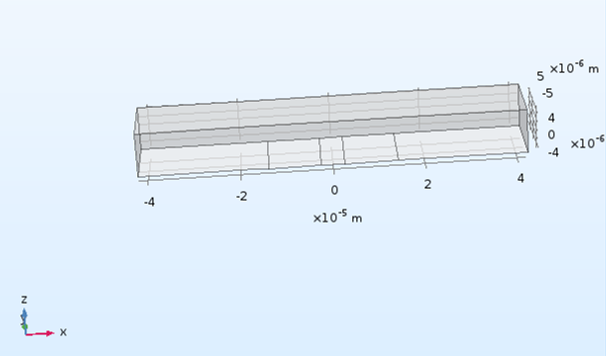
\includegraphics[width=\textwidth]{images/simpleMediumGeometry.png}
        \caption{Simple medium model}
        \label{fig:simple_medium_fea_model}
    \end{subfigure}
    \hfill
    \begin{subfigure}[b]{0.45\textwidth}
        \centering
        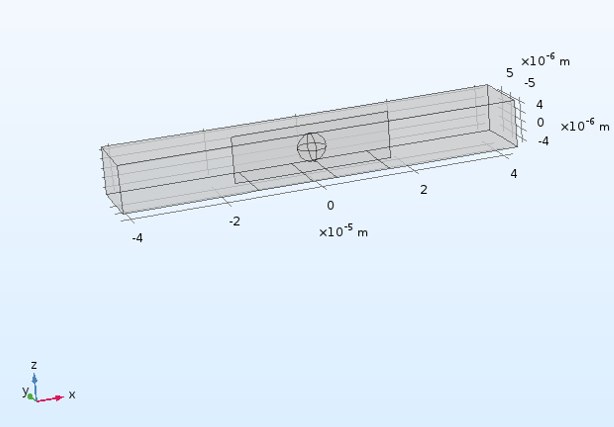
\includegraphics[width=\textwidth]{images/simpleCellGeometry.png}
        \caption{Simple cell model}
        \label{fig:simple_medium_with_cell_fea_model}
    \end{subfigure}
    \\ \vspace{0.3 in}
    \begin{subfigure}[b]{0.45\textwidth}
        \centering
        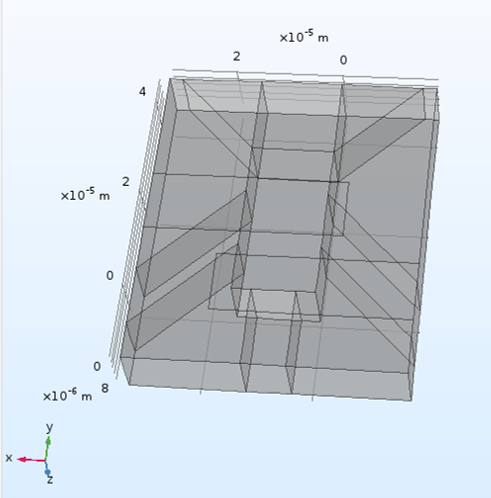
\includegraphics[width=\textwidth]{images/deviceMediumGeometry.png}
        \caption{Device medium model}
        \label{fig:device_medium_fea_model}
    \end{subfigure}
    \hfill
    \begin{subfigure}[b]{0.45\textwidth}
        \centering
        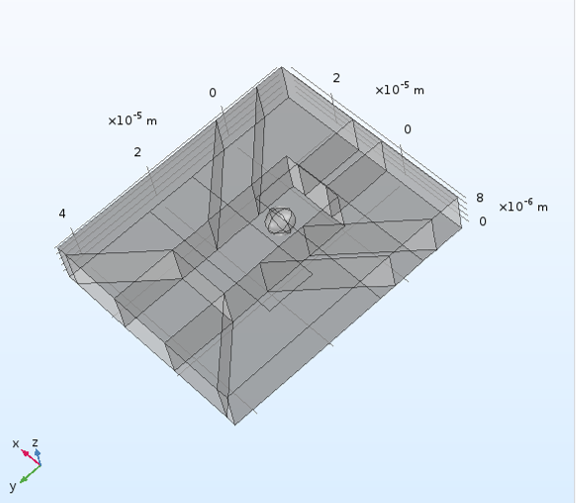
\includegraphics[width=\textwidth]{images/deviceCellGeometry.png}
        \caption{Device cell model}
        \label{fig:device_cell_fea_model}
    \end{subfigure}
    \caption{Finite element analysis models.}
    \label{fig:FEA_models}
\end{figure}


%%% Model Development
\subsection{Model Development}
\par The simple medium, simple cell, device medium, and device cell models were created using COMSOL Multiphyisics FEA software with the electric current physics module. Model development included the specification and implementation in COMSOL of geometry, material properties, and governing physics.

\subsection*{Model Geometry}
\par Two geometries were developed for the impedance spectroscopy models: a basic rectangular electrode cell for the simple models, and an implementation of the impedance spectroscopy device for the device models. The simple geometry is depicted in figure \ref{fig:simple_medium_fea_model} and \ref{fig:simple_medium_with_cell_fea_model}, and the device geometry in figure \ref{fig:device_medium_fea_model} and \ref{fig:device_cell_fea_model}. Dimensioned drawings are presented in figure \ref{fig:simple_model_geometry} and figure \ref{fig: FEA_device_geometry} for the simple and device model respectively.

\begin{figure}[h]
    \centering
    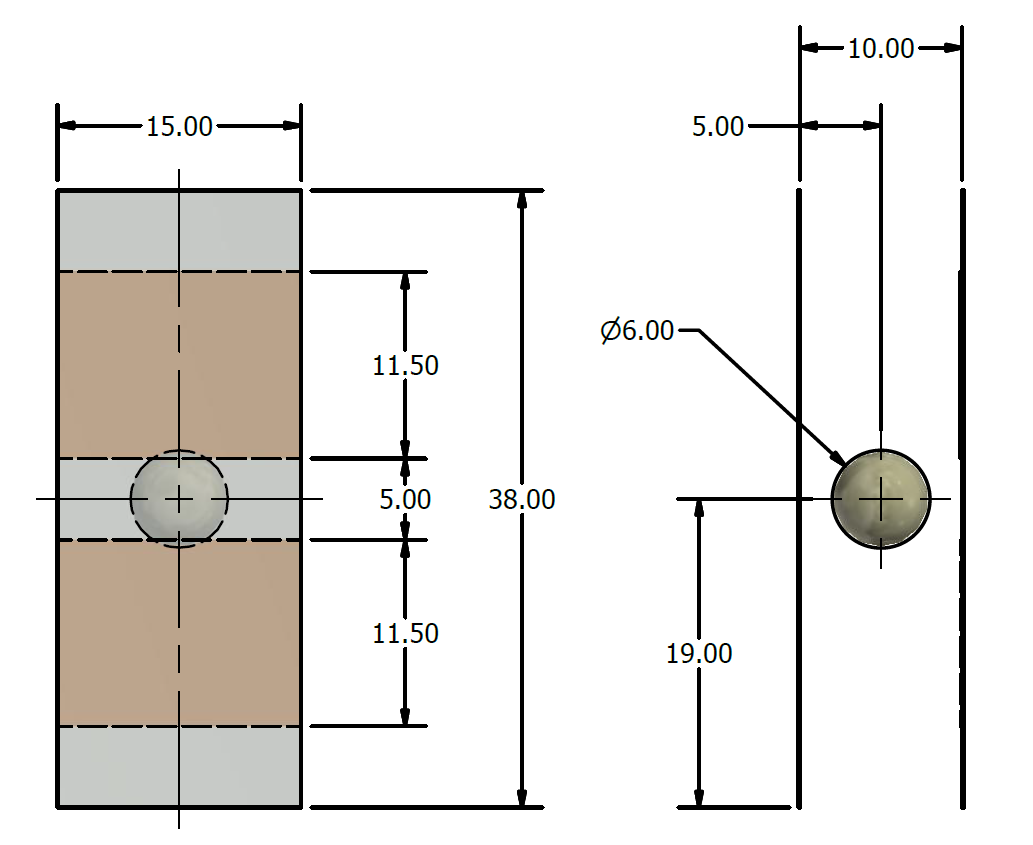
\includegraphics[width=0.7\textwidth]{images/simple_cell_drawing_inventor.png}
    \caption[Simple FEA model geometry.]{Drawing of the Simple FEA models geometry. All units of length are in microns.}
    \label{fig:simple_model_geometry}
\end{figure}


\par In general, the simple geometry attempts to follow two of the assumptions made in the analytic impedance solution with reference to the electrode orientation given in figure \ref{fig:??}:
\begin{enumerate}
    \item The electrode fringe fields are allowed to expand infinitely in the $\hat{\boldsymbol\imath}$ direction (i.e. there is no horizontal insulation).
    \item The electric field has no component in the $\hat{\boldsymbol\jmath}$ direction (i.e. geometry must be uniform in the direction parallel to the electrodes).
\end{enumerate}


\par The simple geometry approximated assumption 1 by making the sensor chamber sufficiently long. An iterative approach determined the sufficient length of the chamber by repeatedly increasing the length of the chamber until the model impedance stabilized to a constant value. At this point, any additional fringe fields permitted by an infinitely long channel was assumed to be negligible. This approach led to an optimal model length of 38 microns. The second assumption was met by creating uniform features in the $\hat{\boldsymbol\jmath}$ direction.


 \begin{figure}[H]
    \centering
    \begin{subfigure}[b]{\textwidth}
      \centering
    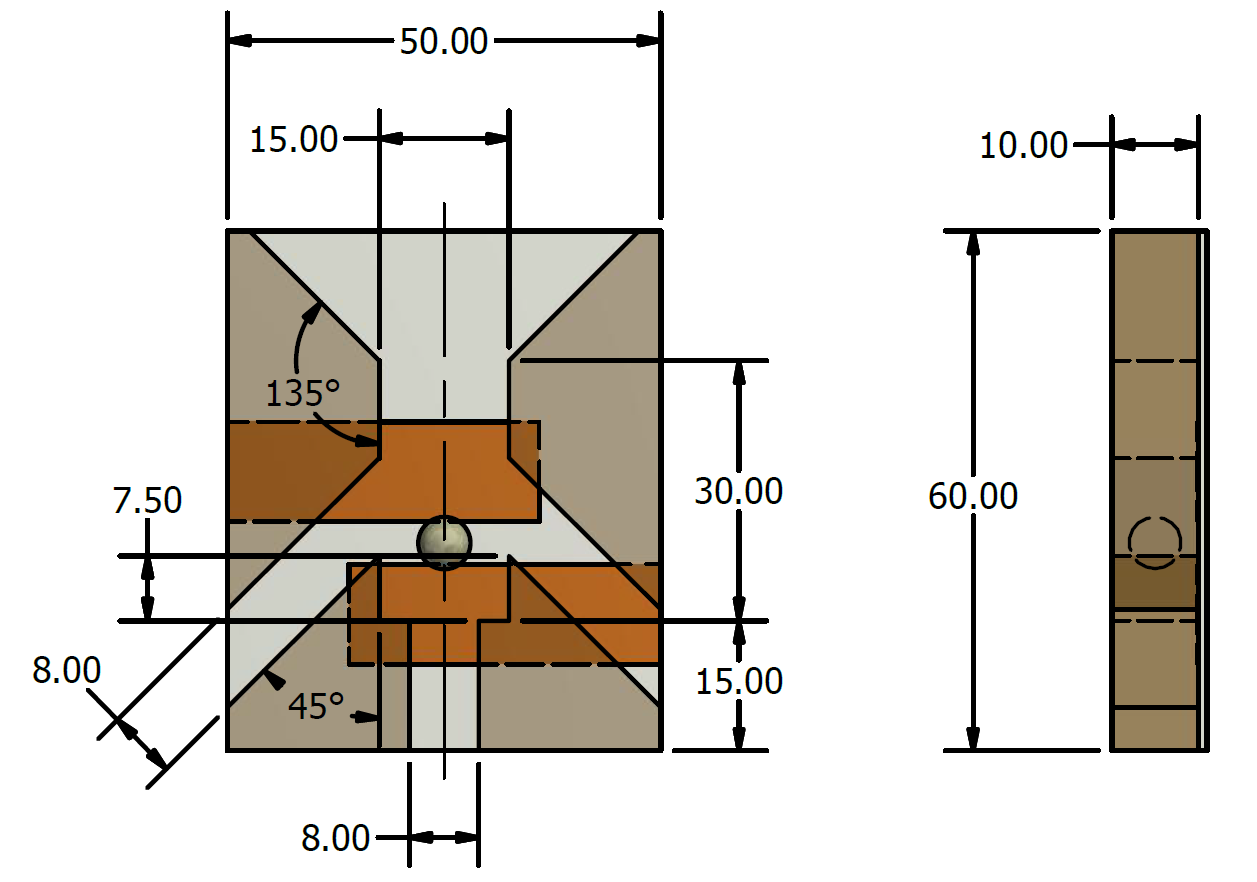
\includegraphics[width=0.6\textwidth]{images/channel_dimensions_inventor.png}
    \caption[]{Drawing of the geometry used in the device FEA model with dimensioned system and PDMS geometry. All dimensions of length in units of microns.}
    \label{fig:device_channel_dimensions_FEA}
    \end{subfigure}
    \\
    \vspace{0.2 in}
    \begin{subfigure}[b]{\textwidth}
        \centering
        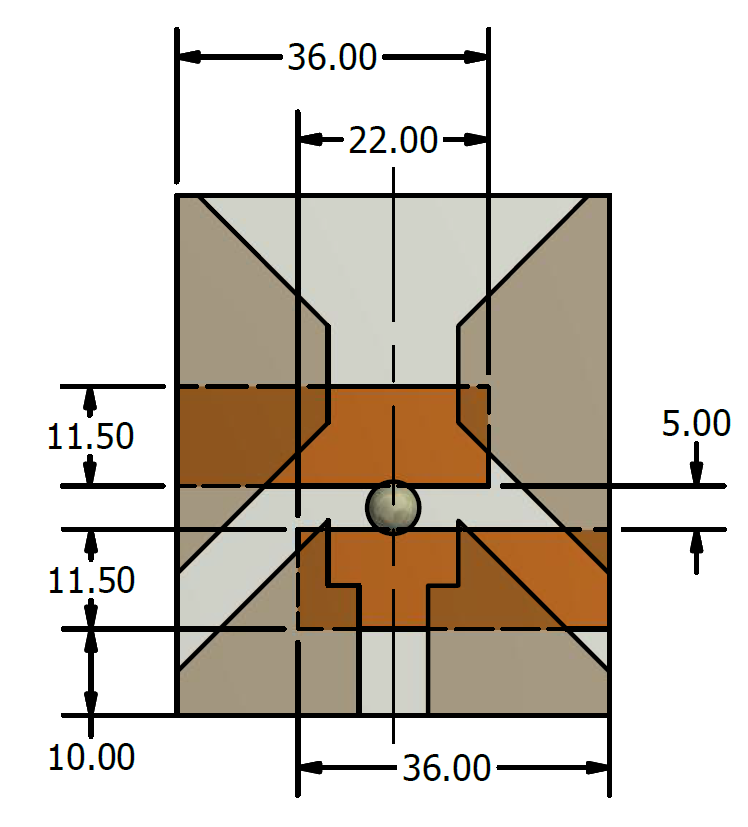
\includegraphics[width=0.4\textwidth]{electrode_dimensions_inventor}
       \caption{Drawing of the geometry used in the Device Medium and Device Cell FEA models with dimensioned electrode geometry. All dimensions of length in units of microns.}
        \label{fig:device_electrode_dimensions_FEA}
    \end{subfigure} 
    \\
    \vspace{0.2 in}
    \begin{subfigure}[b]{\textwidth}
        \centering
        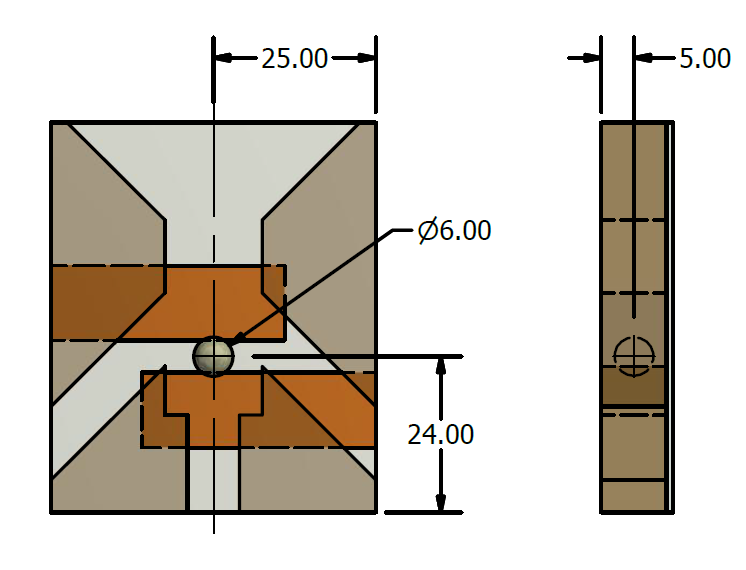
\includegraphics[width=0.55\textwidth]{images/particle_dimension_inventor.png}
        \caption{Drawing of the geometry used in the Device Cell FEA model with dimensioned cell geometry. All dimensions of length in units of microns.}
        \label{fig:device_cell_dimensions_FEA}
    \end{subfigure} 
    \caption[Device FEA model geometry.]{Drawing of the Device FEA geometry models. All dimensions of length are in microns.}
    \label{fig: FEA_device_geometry}
 \end{figure}


\par The device geometry focused on the sensor chamber of the impedance spectroscope device and assumed that the effects of the electrodes far from the chamber are negligible. 


\par The cell version of both geometries includes a cell centered over the electrodes with the cell center 5 microns above the electrodes. The cell was modeled as a 6 $\mu$m diameter sphere of cytoplasm. The 7.5 nm cell membrane is implemented in the physics. 

\par Additional detail in generating the geometry model is presented in appendix \ref{app: comsol_setup}.

\subsection*{Material Properties}
\par The materials used in the FEA models included the medium solution, the cell membrane, cytoplasm, and polydimethylsiloxane (PDMS). For each of these materials materials, the conductivity and relative permittivity were specified and are summarized in table \ref{tab:fea_materials}.

\begin{table}[h]
    \centering
    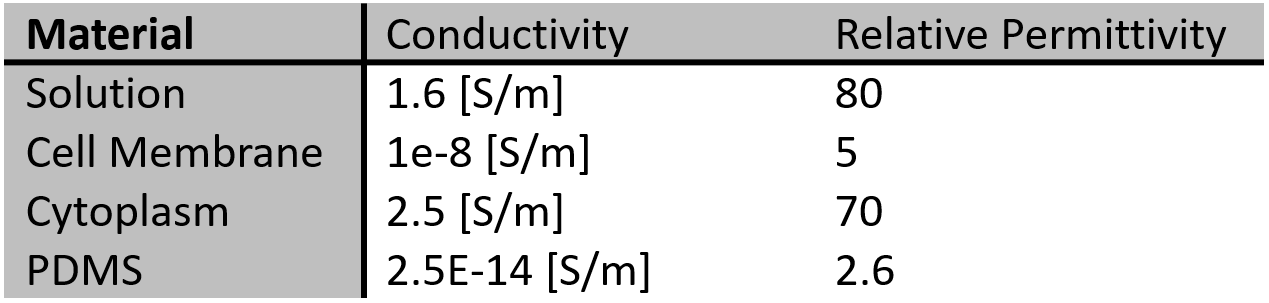
\includegraphics[width=0.75\textwidth]{images/materialpropertiestable.png}
    \caption{Table of material properties.}
    \label{tab:fea_materials}
\end{table}

\subsection*{Physics}
\par The electric current COMSOL interface was to set the physical equations for the models. The governing formula is the equation of continuity:
\begin{equation}
    \boldsymbol\nabla \boldsymbol\cdot \boldsymbol J = -\frac{d\rho}{dt}
\end{equation}

where $-\frac{d\rho}{dt}$ is the rate of change of charge density and $\boldsymbol J$ is the current density expressed as
\begin{equation}
    \boldsymbol J = \sigma\boldsymbol\E + jw\boldsymbol D + \boldsymbol J_e
\end{equation}

where \boldsymbol\E is the electric field, $j$ is $\sqrt{-1}$, $w$ is the angular frequency, $\boldsymbol J_e$ is the externally generated current density, and $\boldsymbol D$ is the electric displacement field. 

\par All exterior bound, except for the electrodes, are modeled as perfect insulators with the boundary condition
\begin{equation}
    \hat{\boldsymbol n} \boldsymbol\cdot \boldsymbol J = 0
\end{equation}

\par The cell membrane was modeled with the contact impedance condition. This is an effective alternative to meshing very thin boundaries. The condition is defined by
\begin{equation}
    \hat{\boldsymbol n} \boldsymbol\cdot \boldsymbol J = \frac{\Tilde{\sigma}}{d_{m}} \Delta V
\end{equation}

where $d_m$ is the thickness of the cell membrane and $\Tilde{\sigma}$ is the complex conductivity expressed as
\begin{equation}
    \Tilde{\sigma} = \sigma + jw\epsilon 
\end{equation}

\par The contact impedance condition only allows current normal to the selected boundary and does not allow current tangentially through the boundary. The condition can be used as an effective approximation to thin and relatively non-conductive domains. In the case of the cell membrane, it is an appropriate approximation. 

\par The low and high potential electrodes were set as the ground ($v=0$) and the applied voltage ($v=v_0$).

\par The impedance of the system was calculated by dividing the input voltage of $v_0 = 1$V by the system system current. The system current was calculated by placing a boundary probe over the ground electrode that integrated the current density over the surface of the electrode. The calculation resulted in the phasor impedance of the electrode cell. 

%%% Mesh Development
\subsection{Mesh Development}

\par The FEA models were meshed with quadratic tetrahedral meshes.  Mesh convergence studies were run on all four models to determine appropriate meshes and to validate that the model is convergent. To improve the simulation efficiency, the mesh was only refined in the regions over the electrodes. 

\par Each convergence study was based on the calculated resistance of the system (i.e impedance at 0 hz), which requires integrating the current density over an electrode to find current. In COMSOL, the default settings using the Electric Current module only provides a discretized spatial gradient to the post-processor. When post-processing calculations use the spatial gradient, the result is highly mesh dependent and can result in greater errors. In the simple medium model, this effect manifested as with non-zero current values through perfectly insulated boundaries and the apparent break down of the continuity equation. As a result, an additional error is added to the calculated impedance and the model will require a greater number of degrees of freedom (DOFs) to converge. The effect can be mitigated by applying weak constraints on the boundaries used for post-processing flux calculations. The weak constraint setting provides the post-processor with additional variables that allow for accurate flux calculations. The effect of weak constraints is illustrated in the convergence study of the simple medium model depicted in figure \ref{fig:simple_medium_convergence}. Weak constraints were used in the simple models, but due to complicated geometry over the electrodes in the device models, COMSOL was unable to compile the simulation with weak constraints and the non-weak constraints were used keeping this shortcoming in mind.

\begin{figure}[h]
    \centering
    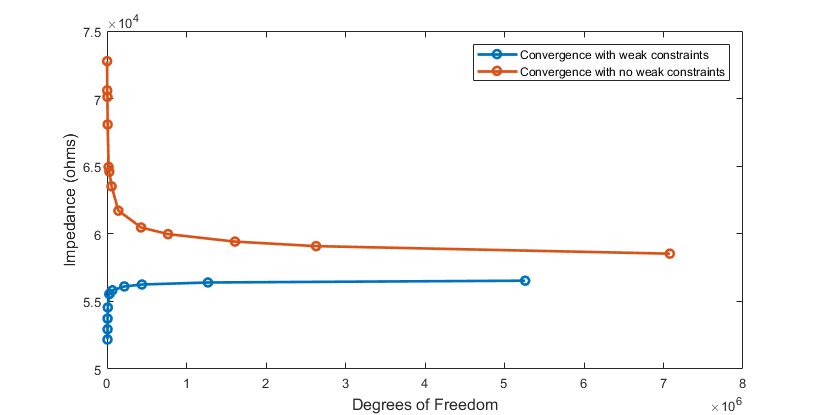
\includegraphics[width=\textwidth]{images/simpeMediumConvergenceNoValidation.png}
    \caption{Simple medium convergence}
    \label{fig:simple_medium_convergence}
\end{figure}


\begin{figure}[h]
    \centering
    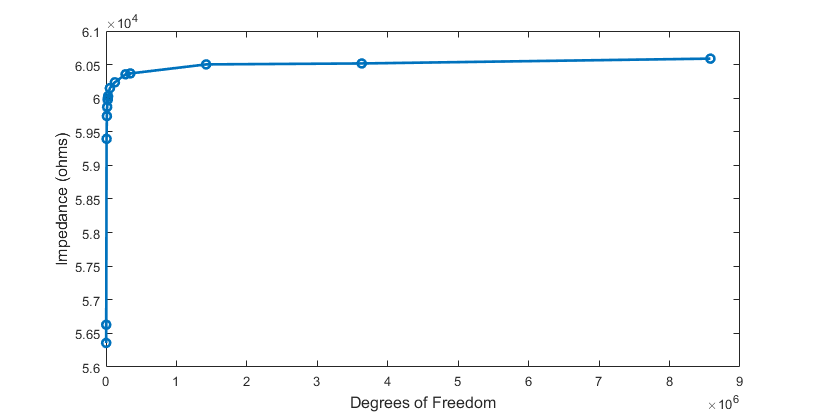
\includegraphics[width=0.9\textwidth]{images/simpleCellConvergence.png}
    \caption{Simple Cell convergence}
    \label{fig:simple_cell_convergence}
\end{figure}
\begin{figure}[h]
    \centering
    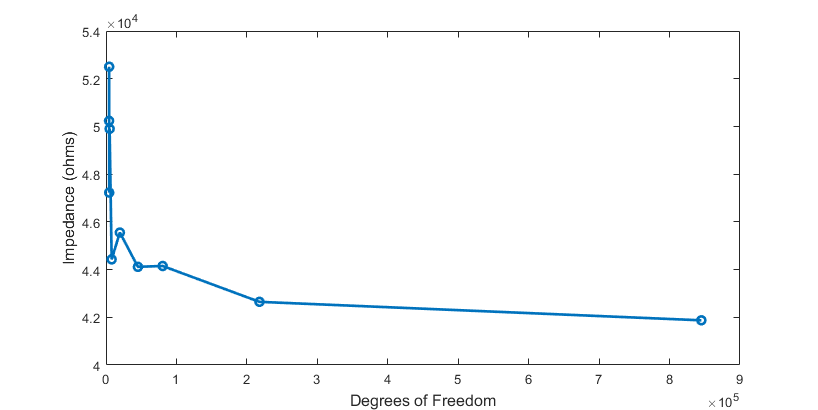
\includegraphics[width=0.9\textwidth]{images/device_medium_convergence.png}
    \caption{Device Medium convergence}
    \label{fig:device_medium_convergence}
\end{figure}
\begin{figure}[H]
    \centering
    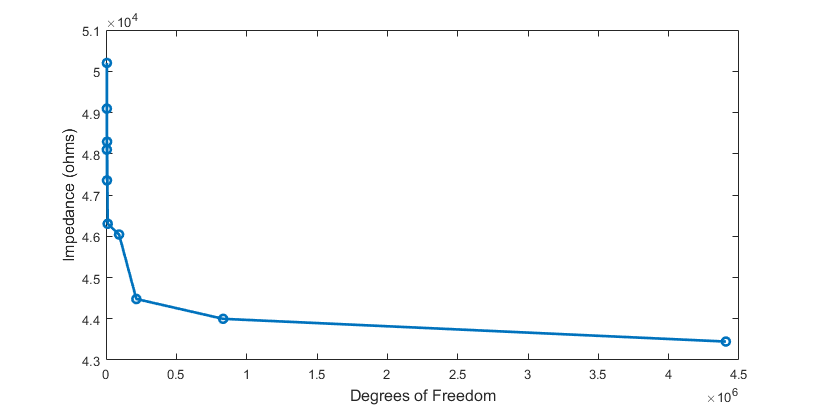
\includegraphics[width=0.9\textwidth]{images/device_cell_convergence.png}
    \caption{Device Cell convergence}
    \label{fig:device_cell_convergence}
\end{figure}

\par The results of the convergence studies are presented in figures \ref{fig:simple_medium_convergence}, \ref{fig:simple_cell_convergence}, \ref{fig:device_medium_convergence}, and \ref{fig:device_cell_convergence}. The meshes corresponding to 2.18E5, 2.785E5, 8.45E5, and 8.33E5 degrees of freedom were chosen for the simple medium, simple cell, device medium, and device cell respectively. The chosen meshes are depicted in figure \ref{fig:FEA_meshes} with mesh descriptions in table \ref{tab: meshStats}. 

\begin{figure}[h]
    \centering
    \begin{subfigure}[b]{0.45\textwidth}
        \centering
        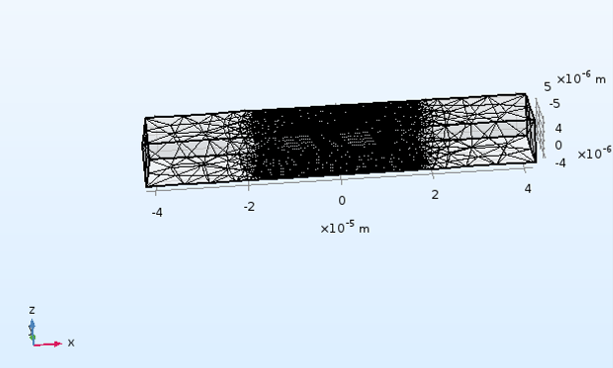
\includegraphics[width=\textwidth]{images/simpleMediumMesh.png}
        \caption{Simple medium mesh}
        \label{fig:simple_medium_mesh}
    \end{subfigure}
    \hfill
    \begin{subfigure}[b]{0.45\textwidth}
        \centering
        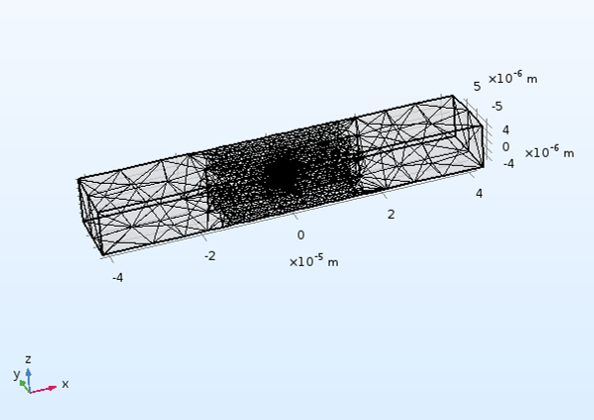
\includegraphics[width=\textwidth]{images/simpleCellMesh.png}
        \caption{Simple cell mesh}
        \label{fig:simple_cell_mesh}
    \end{subfigure}
    \\ \vspace{0.3 in}
    \begin{subfigure}[b]{0.45\textwidth}
        \centering
        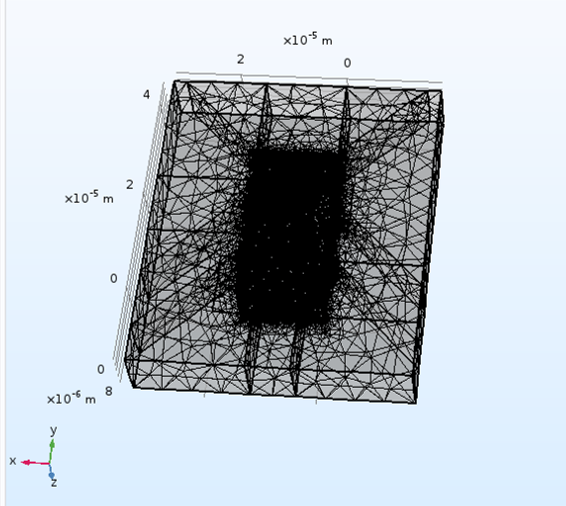
\includegraphics[width=\textwidth]{images/deviceMediumMesh.png}
        \caption{Device medium mesh}
        \label{fig:device_medium_mesh}
    \end{subfigure}
    \hfill
    \begin{subfigure}[b]{0.45\textwidth}
        \centering
        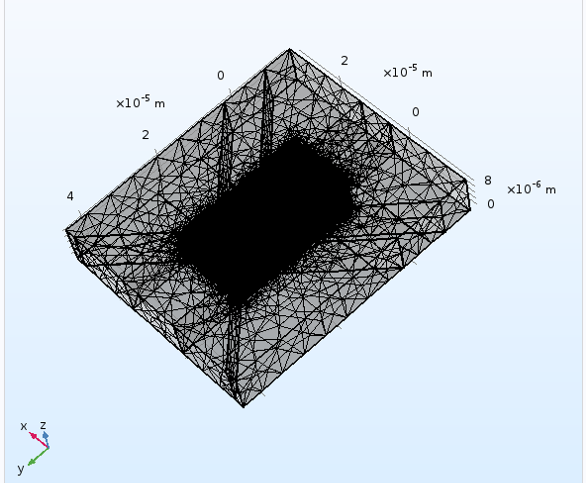
\includegraphics[width=\textwidth]{images/deviceCellMesh.png}
        \caption{Device cell mesh}
        \label{fig:device_cell_mesh}
    \end{subfigure}
    \caption{Finite element analysis models.}
    \label{fig:FEA_meshes}
\end{figure}
\begin{table}[h]
    \centering
    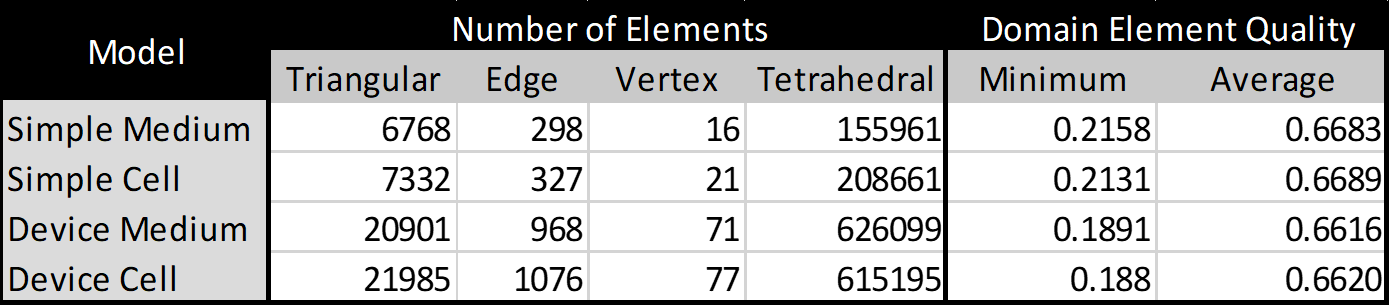
\includegraphics[width=\textwidth]{images/meshStats.png}
    \caption{Caption}
    \label{tab: meshStats}
\end{table}



%%% Validation
\subsection{Model Validation}
\par The FEA models were validated by comparing the analytic impedance solutions to the results of the simple medium and the simple cell models. The analytic solutions were calculated using the the dimensions of the figure \ref{fig:simple_model_geometry}, the material properties in table \ref{tab:fea_materials}, direct current, and utilizing both the traditional and power fractions. The results of the analytic impedance solutions were overlayed on the simple model convergence studies and presented in figure \ref{fig:simple_medium_validation} and \ref{fig:simple_cell_validation}.

\begin{figure}[h]
    \centering
    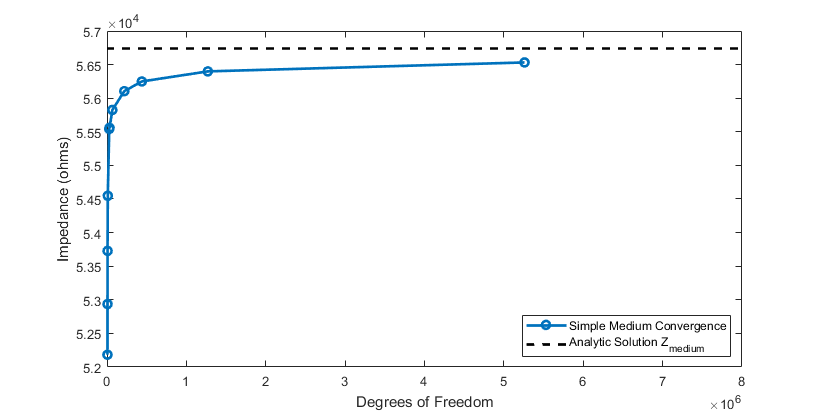
\includegraphics[width=\textwidth]{images/simpeMediumValidation.png}
    \caption{Simple medium validation}
    \label{fig:simple_medium_validation}
\end{figure}

\begin{figure}[H]
    \centering
    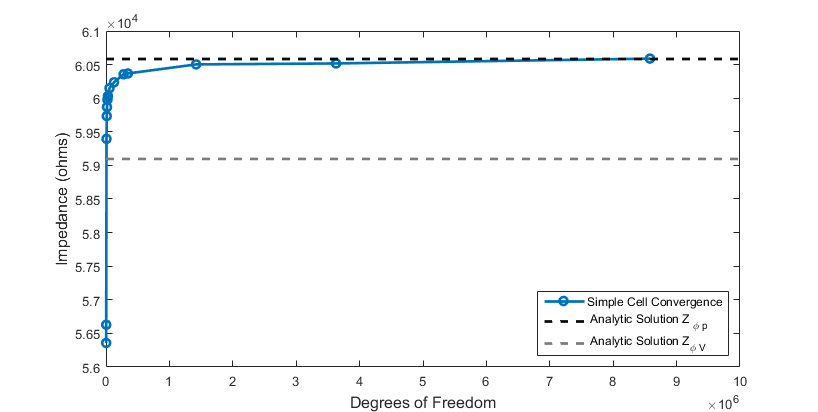
\includegraphics[width=\textwidth]{images/simpleCellValidation.png}
    \caption{Simple Cell validation}
    \label{fig:simple_cell_validation}
\end{figure}


\par A percent error of 0.368\% was calculated for the medium comparison and percent errors of 2.524\% and 0.00990\% were calculated using the traditional and the power volume fraction for the single cell suspension comparisons respectively. By taking the difference of the medium and the single cell suspension impedance, a value more closely related to the cell impedance can be obtained. Percent errors of 58.2\% and 0.148\% were calculated for the traditional and power volume fraction respectively for the difference comparisons.

\par These results validate the simple FEA models and provides strong evidence that extensions of these models (i.e. parametric analysis, frequency sweeps, and the device models) will provide accurate results. In additions, these results highlight how the use of the the adjusted volume fractions are significantly more accurate than the traditional volume fraction (error with power fraction: 0.148\% vs. error with traditional volume fraction: 58.2\%). 






%%%%%%%%%%%%%%%%%%%%%%%%%%%%%%%%%%%
%%%%%%%%  Spice Models  %%%%%%%%%%%
%%%%%%%%%%%%%%%%%%%%%%%%%%%%%%%%%%%
\section{SPICE Circuit Models}
\par  Circuit simulations were developed to validate the IS DAQ system, understand its shortcomings, and explore the I-V and alternative measuremtent circuits. 

\par The circuit models were simulated by leveraging the NGSPICE circuit simulator and interfaced to MATLAB to script model execution and analyze results. By interfacing MATLAB to NGSPICE, greater flexibility allowed for multi-variable parametric analysis, programmatic data analysis, and result presentation. The MATLAB code interface with NGSPICE, and the base Net files are included in appendix \ref{app:spiceModels}. 


$\hat{z}$